% Options for packages loaded elsewhere
\PassOptionsToPackage{unicode}{hyperref}
\PassOptionsToPackage{hyphens}{url}
%
\documentclass[
]{article}
\usepackage{amsmath,amssymb}
\usepackage{iftex}
\ifPDFTeX
  \usepackage[T1]{fontenc}
  \usepackage[utf8]{inputenc}
  \usepackage{textcomp} % provide euro and other symbols
\else % if luatex or xetex
  \usepackage{unicode-math} % this also loads fontspec
  \defaultfontfeatures{Scale=MatchLowercase}
  \defaultfontfeatures[\rmfamily]{Ligatures=TeX,Scale=1}
\fi
\usepackage{lmodern}
\ifPDFTeX\else
  % xetex/luatex font selection
\fi
% Use upquote if available, for straight quotes in verbatim environments
\IfFileExists{upquote.sty}{\usepackage{upquote}}{}
\IfFileExists{microtype.sty}{% use microtype if available
  \usepackage[]{microtype}
  \UseMicrotypeSet[protrusion]{basicmath} % disable protrusion for tt fonts
}{}
\makeatletter
\@ifundefined{KOMAClassName}{% if non-KOMA class
  \IfFileExists{parskip.sty}{%
    \usepackage{parskip}
  }{% else
    \setlength{\parindent}{0pt}
    \setlength{\parskip}{6pt plus 2pt minus 1pt}}
}{% if KOMA class
  \KOMAoptions{parskip=half}}
\makeatother
\usepackage{xcolor}
\usepackage[margin=1in]{geometry}
\usepackage{color}
\usepackage{fancyvrb}
\newcommand{\VerbBar}{|}
\newcommand{\VERB}{\Verb[commandchars=\\\{\}]}
\DefineVerbatimEnvironment{Highlighting}{Verbatim}{commandchars=\\\{\}}
% Add ',fontsize=\small' for more characters per line
\usepackage{framed}
\definecolor{shadecolor}{RGB}{248,248,248}
\newenvironment{Shaded}{\begin{snugshade}}{\end{snugshade}}
\newcommand{\AlertTok}[1]{\textcolor[rgb]{0.94,0.16,0.16}{#1}}
\newcommand{\AnnotationTok}[1]{\textcolor[rgb]{0.56,0.35,0.01}{\textbf{\textit{#1}}}}
\newcommand{\AttributeTok}[1]{\textcolor[rgb]{0.13,0.29,0.53}{#1}}
\newcommand{\BaseNTok}[1]{\textcolor[rgb]{0.00,0.00,0.81}{#1}}
\newcommand{\BuiltInTok}[1]{#1}
\newcommand{\CharTok}[1]{\textcolor[rgb]{0.31,0.60,0.02}{#1}}
\newcommand{\CommentTok}[1]{\textcolor[rgb]{0.56,0.35,0.01}{\textit{#1}}}
\newcommand{\CommentVarTok}[1]{\textcolor[rgb]{0.56,0.35,0.01}{\textbf{\textit{#1}}}}
\newcommand{\ConstantTok}[1]{\textcolor[rgb]{0.56,0.35,0.01}{#1}}
\newcommand{\ControlFlowTok}[1]{\textcolor[rgb]{0.13,0.29,0.53}{\textbf{#1}}}
\newcommand{\DataTypeTok}[1]{\textcolor[rgb]{0.13,0.29,0.53}{#1}}
\newcommand{\DecValTok}[1]{\textcolor[rgb]{0.00,0.00,0.81}{#1}}
\newcommand{\DocumentationTok}[1]{\textcolor[rgb]{0.56,0.35,0.01}{\textbf{\textit{#1}}}}
\newcommand{\ErrorTok}[1]{\textcolor[rgb]{0.64,0.00,0.00}{\textbf{#1}}}
\newcommand{\ExtensionTok}[1]{#1}
\newcommand{\FloatTok}[1]{\textcolor[rgb]{0.00,0.00,0.81}{#1}}
\newcommand{\FunctionTok}[1]{\textcolor[rgb]{0.13,0.29,0.53}{\textbf{#1}}}
\newcommand{\ImportTok}[1]{#1}
\newcommand{\InformationTok}[1]{\textcolor[rgb]{0.56,0.35,0.01}{\textbf{\textit{#1}}}}
\newcommand{\KeywordTok}[1]{\textcolor[rgb]{0.13,0.29,0.53}{\textbf{#1}}}
\newcommand{\NormalTok}[1]{#1}
\newcommand{\OperatorTok}[1]{\textcolor[rgb]{0.81,0.36,0.00}{\textbf{#1}}}
\newcommand{\OtherTok}[1]{\textcolor[rgb]{0.56,0.35,0.01}{#1}}
\newcommand{\PreprocessorTok}[1]{\textcolor[rgb]{0.56,0.35,0.01}{\textit{#1}}}
\newcommand{\RegionMarkerTok}[1]{#1}
\newcommand{\SpecialCharTok}[1]{\textcolor[rgb]{0.81,0.36,0.00}{\textbf{#1}}}
\newcommand{\SpecialStringTok}[1]{\textcolor[rgb]{0.31,0.60,0.02}{#1}}
\newcommand{\StringTok}[1]{\textcolor[rgb]{0.31,0.60,0.02}{#1}}
\newcommand{\VariableTok}[1]{\textcolor[rgb]{0.00,0.00,0.00}{#1}}
\newcommand{\VerbatimStringTok}[1]{\textcolor[rgb]{0.31,0.60,0.02}{#1}}
\newcommand{\WarningTok}[1]{\textcolor[rgb]{0.56,0.35,0.01}{\textbf{\textit{#1}}}}
\usepackage{graphicx}
\makeatletter
\def\maxwidth{\ifdim\Gin@nat@width>\linewidth\linewidth\else\Gin@nat@width\fi}
\def\maxheight{\ifdim\Gin@nat@height>\textheight\textheight\else\Gin@nat@height\fi}
\makeatother
% Scale images if necessary, so that they will not overflow the page
% margins by default, and it is still possible to overwrite the defaults
% using explicit options in \includegraphics[width, height, ...]{}
\setkeys{Gin}{width=\maxwidth,height=\maxheight,keepaspectratio}
% Set default figure placement to htbp
\makeatletter
\def\fps@figure{htbp}
\makeatother
\setlength{\emergencystretch}{3em} % prevent overfull lines
\providecommand{\tightlist}{%
  \setlength{\itemsep}{0pt}\setlength{\parskip}{0pt}}
\setcounter{secnumdepth}{-\maxdimen} % remove section numbering
\ifLuaTeX
  \usepackage{selnolig}  % disable illegal ligatures
\fi
\usepackage{bookmark}
\IfFileExists{xurl.sty}{\usepackage{xurl}}{} % add URL line breaks if available
\urlstyle{same}
\hypersetup{
  pdftitle={Final Project STAT167},
  pdfauthor={Group: Statistically Speaking; Shreya Mohan, Kalyani Mantirraju, Crystal Arevalo, Karen Alvarez, Mason Lam, Eric Yang},
  hidelinks,
  pdfcreator={LaTeX via pandoc}}

\title{Final Project STAT167}
\author{Group: Statistically Speaking \and Shreya Mohan, Kalyani
Mantirraju, Crystal Arevalo, Karen Alvarez, Mason Lam, Eric Yang}
\date{06/02/2025}

\begin{document}
\maketitle

\subsection{Libraries}\label{libraries}

\begin{Shaded}
\begin{Highlighting}[]
\CommentTok{\#install.packages("dunn.test")}
\CommentTok{\#install.packages("multcomp")}
\CommentTok{\# install.packages("nortest")}
\CommentTok{\# install.packages("rstatix")}
\CommentTok{\# install.packages("mgcv")}
\FunctionTok{library}\NormalTok{(mgcv)}
\FunctionTok{library}\NormalTok{(rstatix)}
\FunctionTok{library}\NormalTok{(nycflights13)}
\FunctionTok{library}\NormalTok{(tidyverse)}
\FunctionTok{library}\NormalTok{(car)}
\FunctionTok{library}\NormalTok{(dunn.test)}
\FunctionTok{library}\NormalTok{(gridExtra)}
\FunctionTok{library}\NormalTok{(nycflights13)}
\FunctionTok{library}\NormalTok{(dplyr)}
\FunctionTok{library}\NormalTok{(ggplot2)}
\FunctionTok{library}\NormalTok{(tidyr)}
\FunctionTok{library}\NormalTok{(broom)}
\FunctionTok{library}\NormalTok{(car) }
\FunctionTok{library}\NormalTok{(multcomp)}
\FunctionTok{library}\NormalTok{(nortest)}
\FunctionTok{library}\NormalTok{(rstatix)}
\FunctionTok{library}\NormalTok{(dplyr)}
\FunctionTok{library}\NormalTok{(boot)}
\end{Highlighting}
\end{Shaded}

\section{Project Description:}\label{project-description}

The primary goal of this research is to explore factors influencing
flight delays from New City airports in 2013.

\subsection{Problem Statement and
Motivation}\label{problem-statement-and-motivation}

Understanding factors that contribute to flight delays is critical for
informing Federal Aviation Administration (FAA) policies and guiding
airlines and airports in improving operational efficiency, enhancing
weather preparedness, and reducing delays through controllable factors.
By analyzing weather conditions, airline differences, holiday effects,
fleet age, and airport specific challenges, this research can provide
data-driven insights to optimize air travel and ensure compliance with
aviation regulations in heavily congested areas like New York City.

\subsection{Research Questions}\label{research-questions}

\begin{enumerate}
\def\labelenumi{\arabic{enumi}.}
\tightlist
\item
  How do weather conditions affect flight delays?
\item
  How do differences between airlines influence flight delays?
\item
  Are delays more frequent during major holidays?
\item
  Does the age of the plane affect flight delays?
\item
  How do environmental factors like humidity, visibility, and wind
  affect flight delays?
\end{enumerate}

\section{Datasets}\label{datasets}

\subsection{1. Flights dataset: All flights that departed from NYC in
2013}\label{flights-dataset-all-flights-that-departed-from-nyc-in-2013}

\subsubsection{Variables:}\label{variables}

\begin{itemize}
\tightlist
\item
  flights ( year, month, day, dep\_time, arr\_time, sched\_dep\_time,
  sched\_arr\_time, dep\_delay, arr\_delay, carrier, origin, dest,
  air\_time, distance, time\_hour )

  \begin{itemize}
  \tightlist
  \item
    year, month, day : date of departure
  \item
    dep\_time, arr\_time : actual departure and arrival times in HHMM
  \item
    sched\_dep\_time, sched\_arr\_time : scheduled departure and arrival
    times in HHMM
  \item
    dep\_delay, arr\_delay : departure and arrival delays in minutes
  \item
    carrier : two letter carrier abbreviation of the carrier
  \item
    origin, dest : origin and destination
  \item
    air\_time : amount of time spent in air in minutes
  \item
    distance : distance between airport in miles
  \item
    time\_hour : scheduled date and hour of the flight as POSIXct date
  \end{itemize}
\end{itemize}

\subsection{2. Airlines dataset: Translation between two letter carrier
codes and
names}\label{airlines-dataset-translation-between-two-letter-carrier-codes-and-names}

\subsubsection{Variables:}\label{variables-1}

\begin{itemize}
\tightlist
\item
  airlines ( carrier, name )

  \begin{itemize}
  \tightlist
  \item
    carrier : two-letter abbreviation of the airlines
  \item
    name : full name of the airlines
  \end{itemize}
\end{itemize}

\subsection{3. Airports dataset: Airport names and
locations}\label{airports-dataset-airport-names-and-locations}

\begin{Shaded}
\begin{Highlighting}[]
\FunctionTok{head}\NormalTok{(airports)}
\end{Highlighting}
\end{Shaded}

\begin{verbatim}
## # A tibble: 6 x 8
##   faa   name                             lat   lon   alt    tz dst   tzone      
##   <chr> <chr>                          <dbl> <dbl> <dbl> <dbl> <chr> <chr>      
## 1 04G   Lansdowne Airport               41.1 -80.6  1044    -5 A     America/Ne~
## 2 06A   Moton Field Municipal Airport   32.5 -85.7   264    -6 A     America/Ch~
## 3 06C   Schaumburg Regional             42.0 -88.1   801    -6 A     America/Ch~
## 4 06N   Randall Airport                 41.4 -74.4   523    -5 A     America/Ne~
## 5 09J   Jekyll Island Airport           31.1 -81.4    11    -5 A     America/Ne~
## 6 0A9   Elizabethton Municipal Airport  36.4 -82.2  1593    -5 A     America/Ne~
\end{verbatim}

\begin{Shaded}
\begin{Highlighting}[]
\FunctionTok{names}\NormalTok{(airports)}
\end{Highlighting}
\end{Shaded}

\begin{verbatim}
## [1] "faa"   "name"  "lat"   "lon"   "alt"   "tz"    "dst"   "tzone"
\end{verbatim}

\begin{Shaded}
\begin{Highlighting}[]
\FunctionTok{str}\NormalTok{(airports)}
\end{Highlighting}
\end{Shaded}

\begin{verbatim}
## tibble [1,458 x 8] (S3: tbl_df/tbl/data.frame)
##  $ faa  : chr [1:1458] "04G" "06A" "06C" "06N" ...
##  $ name : chr [1:1458] "Lansdowne Airport" "Moton Field Municipal Airport" "Schaumburg Regional" "Randall Airport" ...
##  $ lat  : num [1:1458] 41.1 32.5 42 41.4 31.1 ...
##  $ lon  : num [1:1458] -80.6 -85.7 -88.1 -74.4 -81.4 ...
##  $ alt  : num [1:1458] 1044 264 801 523 11 ...
##  $ tz   : num [1:1458] -5 -6 -6 -5 -5 -5 -5 -5 -5 -8 ...
##  $ dst  : chr [1:1458] "A" "A" "A" "A" ...
##  $ tzone: chr [1:1458] "America/New_York" "America/Chicago" "America/Chicago" "America/New_York" ...
##  - attr(*, "spec")=
##   .. cols(
##   ..   id = col_double(),
##   ..   name = col_character(),
##   ..   city = col_character(),
##   ..   country = col_character(),
##   ..   faa = col_character(),
##   ..   icao = col_character(),
##   ..   lat = col_double(),
##   ..   lon = col_double(),
##   ..   alt = col_double(),
##   ..   tz = col_double(),
##   ..   dst = col_character(),
##   ..   tzone = col_character()
##   .. )
\end{verbatim}

\begin{Shaded}
\begin{Highlighting}[]
\FunctionTok{glimpse}\NormalTok{(airports)}
\end{Highlighting}
\end{Shaded}

\begin{verbatim}
## Rows: 1,458
## Columns: 8
## $ faa   <chr> "04G", "06A", "06C", "06N", "09J", "0A9", "0G6", "0G7", "0P2", "~
## $ name  <chr> "Lansdowne Airport", "Moton Field Municipal Airport", "Schaumbur~
## $ lat   <dbl> 41.13047, 32.46057, 41.98934, 41.43191, 31.07447, 36.37122, 41.4~
## $ lon   <dbl> -80.61958, -85.68003, -88.10124, -74.39156, -81.42778, -82.17342~
## $ alt   <dbl> 1044, 264, 801, 523, 11, 1593, 730, 492, 1000, 108, 409, 875, 10~
## $ tz    <dbl> -5, -6, -6, -5, -5, -5, -5, -5, -5, -8, -5, -6, -5, -5, -5, -5, ~
## $ dst   <chr> "A", "A", "A", "A", "A", "A", "A", "A", "U", "A", "A", "U", "A",~
## $ tzone <chr> "America/New_York", "America/Chicago", "America/Chicago", "Ameri~
\end{verbatim}

\subsubsection{Variables:}\label{variables-2}

\begin{itemize}
\tightlist
\item
  airports ( faa, name, lat, lon )

  \begin{itemize}
  \tightlist
  \item
    faa : FAA airport code
  \item
    name : usual name of the airport
  \item
    lat, lon : location of airport
  \end{itemize}
\end{itemize}

\subsection{4. Planes dataset: Construction information about each
plane}\label{planes-dataset-construction-information-about-each-plane}

\subsubsection{Variables:}\label{variables-3}

\begin{itemize}
\tightlist
\item
  planes ( year, type, manufacturer, model, engines, seats, speed,
  engine )

  \begin{itemize}
  \tightlist
  \item
    year : year manufactured
  \item
    type : type of plane
  \item
    manufacturer, model : manufacturer and model
  \item
    engines, seats : number of engines and seats
  \item
    speed : average cruising speed in mph
  \item
    engine : type in engine
  \end{itemize}
\end{itemize}

\subsection{5. Weather dataset: Hourly meterological data for each
airport}\label{weather-dataset-hourly-meterological-data-for-each-airport}

\subsubsection{Variables:}\label{variables-4}

\begin{itemize}
\tightlist
\item
  weather ( origin, year, month, day, hour, temp, dewp, humid,
  wind\_dir, wind\_speed, wind\_gust, precip, pressure, visib,
  time\_hour )

  \begin{itemize}
  \tightlist
  \item
    origin : weather station
  \item
    year, month, day, hour : time of recording
  \item
    temp, dewp : temperature and dew point in Fahrenheit
  \item
    humid : relative humidity
  \item
    wind\_dir, wind\_speed, wind\_gust : wind direction in degrees, wind
    speed and gust in mph
  \item
    precip : precipitation in inches
  \item
    pressure : sea level pressure in millibars
  \item
    visib : visibility in miles
  \item
    time\_hour : date and hour of the recording as POSIXct date
  \end{itemize}
\end{itemize}

\newpage
\begin{center}
\section*{Exploratory Data Analysis}
\end{center}

\subsection{Planes Dataset EDA}\label{planes-dataset-eda}

\begin{verbatim}
## 
## Missing values per column:
\end{verbatim}

\begin{verbatim}
##      tailnum         year         type manufacturer        model      engines 
##            0           70            0            0            0            0 
##        seats        speed       engine 
##            0         3299            0
\end{verbatim}

\begin{verbatim}
## 
## Column types and structure:
\end{verbatim}

\begin{verbatim}
## Rows: 3,322
## Columns: 9
## $ tailnum      <chr> "N10156", "N102UW", "N103US", "N104UW", "N10575", "N105UW~
## $ year         <int> 2004, 1998, 1999, 1999, 2002, 1999, 1999, 1999, 1999, 199~
## $ type         <chr> "Fixed wing multi engine", "Fixed wing multi engine", "Fi~
## $ manufacturer <chr> "EMBRAER", "AIRBUS INDUSTRIE", "AIRBUS INDUSTRIE", "AIRBU~
## $ model        <chr> "EMB-145XR", "A320-214", "A320-214", "A320-214", "EMB-145~
## $ engines      <int> 2, 2, 2, 2, 2, 2, 2, 2, 2, 2, 2, 2, 2, 2, 2, 2, 2, 2, 2, ~
## $ seats        <int> 55, 182, 182, 182, 55, 182, 182, 182, 182, 182, 55, 55, 5~
## $ speed        <int> NA, NA, NA, NA, NA, NA, NA, NA, NA, NA, NA, NA, NA, NA, N~
## $ engine       <chr> "Turbo-fan", "Turbo-fan", "Turbo-fan", "Turbo-fan", "Turb~
## # A tibble: 3,322 x 9
##    tailnum  year type              manufacturer model engines seats speed engine
##    <chr>   <int> <chr>             <chr>        <chr>   <int> <int> <int> <chr> 
##  1 N10156   2004 Fixed wing multi~ EMBRAER      EMB-~       2    55    NA Turbo~
##  2 N102UW   1998 Fixed wing multi~ AIRBUS INDU~ A320~       2   182    NA Turbo~
##  3 N103US   1999 Fixed wing multi~ AIRBUS INDU~ A320~       2   182    NA Turbo~
##  4 N104UW   1999 Fixed wing multi~ AIRBUS INDU~ A320~       2   182    NA Turbo~
##  5 N10575   2002 Fixed wing multi~ EMBRAER      EMB-~       2    55    NA Turbo~
##  6 N105UW   1999 Fixed wing multi~ AIRBUS INDU~ A320~       2   182    NA Turbo~
##  7 N107US   1999 Fixed wing multi~ AIRBUS INDU~ A320~       2   182    NA Turbo~
##  8 N108UW   1999 Fixed wing multi~ AIRBUS INDU~ A320~       2   182    NA Turbo~
##  9 N109UW   1999 Fixed wing multi~ AIRBUS INDU~ A320~       2   182    NA Turbo~
## 10 N110UW   1999 Fixed wing multi~ AIRBUS INDU~ A320~       2   182    NA Turbo~
## # i 3,312 more rows
\end{verbatim}

\begin{verbatim}
## 
## First few rows:
\end{verbatim}

\begin{verbatim}
## # A tibble: 6 x 9
##   tailnum  year type               manufacturer model engines seats speed engine
##   <chr>   <int> <chr>              <chr>        <chr>   <int> <int> <int> <chr> 
## 1 N10156   2004 Fixed wing multi ~ EMBRAER      EMB-~       2    55    NA Turbo~
## 2 N102UW   1998 Fixed wing multi ~ AIRBUS INDU~ A320~       2   182    NA Turbo~
## 3 N103US   1999 Fixed wing multi ~ AIRBUS INDU~ A320~       2   182    NA Turbo~
## 4 N104UW   1999 Fixed wing multi ~ AIRBUS INDU~ A320~       2   182    NA Turbo~
## 5 N10575   2002 Fixed wing multi ~ EMBRAER      EMB-~       2    55    NA Turbo~
## 6 N105UW   1999 Fixed wing multi ~ AIRBUS INDU~ A320~       2   182    NA Turbo~
\end{verbatim}

\begin{verbatim}
## 
## Summary statistics:
\end{verbatim}

\begin{verbatim}
##    tailnum               year          type           manufacturer      
##  Length:3322        Min.   :1956   Length:3322        Length:3322       
##  Class :character   1st Qu.:1997   Class :character   Class :character  
##  Mode  :character   Median :2001   Mode  :character   Mode  :character  
##                     Mean   :2000                                        
##                     3rd Qu.:2005                                        
##                     Max.   :2013                                        
##                     NA's   :70                                          
##     model              engines          seats           speed      
##  Length:3322        Min.   :1.000   Min.   :  2.0   Min.   : 90.0  
##  Class :character   1st Qu.:2.000   1st Qu.:140.0   1st Qu.:107.5  
##  Mode  :character   Median :2.000   Median :149.0   Median :162.0  
##                     Mean   :1.995   Mean   :154.3   Mean   :236.8  
##                     3rd Qu.:2.000   3rd Qu.:182.0   3rd Qu.:432.0  
##                     Max.   :4.000   Max.   :450.0   Max.   :432.0  
##                                                     NA's   :3299   
##     engine         
##  Length:3322       
##  Class :character  
##  Mode  :character  
##                    
##                    
##                    
## 
\end{verbatim}

\begin{verbatim}
## Selecting by n
\end{verbatim}

\includegraphics{6-StatistciallySpeaking_files/figure-latex/unnamed-chunk-4-1.pdf}

The visualization above shows the top 10 plane manufacturers present in
the data-set. Boeing has the largest amount of planes with approximately
1750 planes, and Airbus has the second most with approximately 400
planes.

\begin{verbatim}
## Warning: Removed 70 rows containing non-finite outside the scale range
## (`stat_bin()`).
\end{verbatim}

\includegraphics{6-StatistciallySpeaking_files/figure-latex/unnamed-chunk-5-1.pdf}

This histogram shows the distribution of plane manufacture years, with
the majority of planes built between the mid-1990s and early 2000s.
There is a notable peak around the year 2000, indicating a surge in
plane production during that period.

\subsection{Airlines Dataset EDA}\label{airlines-dataset-eda}

Dimensions and column names of the airlines dataset

\begin{verbatim}
## 
## Missing values per column:
\end{verbatim}

\begin{verbatim}
## carrier    name 
##       0       0
\end{verbatim}

\begin{verbatim}
## 
## Column types and structure:
\end{verbatim}

\begin{verbatim}
## Rows: 16
## Columns: 2
## $ carrier <chr> "9E", "AA", "AS", "B6", "DL", "EV", "F9", "FL", "HA", "MQ", "O~
## $ name    <chr> "Endeavor Air Inc.", "American Airlines Inc.", "Alaska Airline~
## # A tibble: 16 x 2
##    carrier name                       
##    <chr>   <chr>                      
##  1 9E      Endeavor Air Inc.          
##  2 AA      American Airlines Inc.     
##  3 AS      Alaska Airlines Inc.       
##  4 B6      JetBlue Airways            
##  5 DL      Delta Air Lines Inc.       
##  6 EV      ExpressJet Airlines Inc.   
##  7 F9      Frontier Airlines Inc.     
##  8 FL      AirTran Airways Corporation
##  9 HA      Hawaiian Airlines Inc.     
## 10 MQ      Envoy Air                  
## 11 OO      SkyWest Airlines Inc.      
## 12 UA      United Air Lines Inc.      
## 13 US      US Airways Inc.            
## 14 VX      Virgin America             
## 15 WN      Southwest Airlines Co.     
## 16 YV      Mesa Airlines Inc.
\end{verbatim}

\begin{verbatim}
## 
## First few rows:
\end{verbatim}

\begin{verbatim}
## # A tibble: 6 x 2
##   carrier name                    
##   <chr>   <chr>                   
## 1 9E      Endeavor Air Inc.       
## 2 AA      American Airlines Inc.  
## 3 AS      Alaska Airlines Inc.    
## 4 B6      JetBlue Airways         
## 5 DL      Delta Air Lines Inc.    
## 6 EV      ExpressJet Airlines Inc.
\end{verbatim}

\begin{verbatim}
## 
## Summary statistics:
\end{verbatim}

\begin{verbatim}
##    carrier              name          
##  Length:16          Length:16         
##  Class :character   Class :character  
##  Mode  :character   Mode  :character
\end{verbatim}

Viewing all the Unique Airlines:

\begin{Shaded}
\begin{Highlighting}[]
\NormalTok{airlines }\SpecialCharTok{\%\textgreater{}\%}
  \FunctionTok{arrange}\NormalTok{(name)}
\end{Highlighting}
\end{Shaded}

\begin{verbatim}
## # A tibble: 16 x 2
##    carrier name                       
##    <chr>   <chr>                      
##  1 FL      AirTran Airways Corporation
##  2 AS      Alaska Airlines Inc.       
##  3 AA      American Airlines Inc.     
##  4 DL      Delta Air Lines Inc.       
##  5 9E      Endeavor Air Inc.          
##  6 MQ      Envoy Air                  
##  7 EV      ExpressJet Airlines Inc.   
##  8 F9      Frontier Airlines Inc.     
##  9 HA      Hawaiian Airlines Inc.     
## 10 B6      JetBlue Airways            
## 11 YV      Mesa Airlines Inc.         
## 12 OO      SkyWest Airlines Inc.      
## 13 WN      Southwest Airlines Co.     
## 14 US      US Airways Inc.            
## 15 UA      United Air Lines Inc.      
## 16 VX      Virgin America
\end{verbatim}

\begin{Shaded}
\begin{Highlighting}[]
\CommentTok{\# Join flights and airline names}
\NormalTok{flights\_airlines }\OtherTok{\textless{}{-}}\NormalTok{ flights }\SpecialCharTok{\%\textgreater{}\%}
  \FunctionTok{left\_join}\NormalTok{(airlines, }\AttributeTok{by =} \StringTok{"carrier"}\NormalTok{)}

\CommentTok{\# Average delay metrics}
\NormalTok{avg\_delays }\OtherTok{\textless{}{-}}\NormalTok{ flights\_airlines }\SpecialCharTok{\%\textgreater{}\%}
  \FunctionTok{group\_by}\NormalTok{(name) }\SpecialCharTok{\%\textgreater{}\%}
  \FunctionTok{summarise}\NormalTok{(}
    \AttributeTok{avg\_dep\_delay =} \FunctionTok{mean}\NormalTok{(dep\_delay, }\AttributeTok{na.rm =} \ConstantTok{TRUE}\NormalTok{),}
    \AttributeTok{avg\_arr\_delay =} \FunctionTok{mean}\NormalTok{(arr\_delay, }\AttributeTok{na.rm =} \ConstantTok{TRUE}\NormalTok{),}
    \AttributeTok{flights =} \FunctionTok{n}\NormalTok{()}
\NormalTok{  )}

\CommentTok{\# Plot: Departure Delay}
\FunctionTok{ggplot}\NormalTok{(avg\_delays, }\FunctionTok{aes}\NormalTok{(}\AttributeTok{x =} \FunctionTok{reorder}\NormalTok{(name, avg\_dep\_delay), }\AttributeTok{y =}\NormalTok{ avg\_dep\_delay)) }\SpecialCharTok{+}
  \FunctionTok{geom\_col}\NormalTok{(}\AttributeTok{fill =} \StringTok{"tomato"}\NormalTok{) }\SpecialCharTok{+}
  \FunctionTok{coord\_flip}\NormalTok{() }\SpecialCharTok{+}
  \FunctionTok{labs}\NormalTok{(}
    \AttributeTok{title =} \StringTok{"Average Departure Delay by Airline"}\NormalTok{,}
    \AttributeTok{x =} \StringTok{"Airline"}\NormalTok{,}
    \AttributeTok{y =} \StringTok{"Avg Departure Delay (min)"}
\NormalTok{  )}
\end{Highlighting}
\end{Shaded}

\includegraphics{6-StatistciallySpeaking_files/figure-latex/unnamed-chunk-8-1.pdf}

We can see that on average, Frontier Airlines has the most departure
delay at around 20 min, with ExpressJet roughly around the same 20
minutes. Less than half the Airlines seem to be past the 13 minute delay
mark.

\begin{Shaded}
\begin{Highlighting}[]
\NormalTok{cancel\_rate }\OtherTok{\textless{}{-}}\NormalTok{ flights\_airlines }\SpecialCharTok{\%\textgreater{}\%}
  \FunctionTok{mutate}\NormalTok{(}\AttributeTok{cancelled =} \FunctionTok{is.na}\NormalTok{(dep\_delay)) }\SpecialCharTok{\%\textgreater{}\%}
  \FunctionTok{group\_by}\NormalTok{(name) }\SpecialCharTok{\%\textgreater{}\%}
  \FunctionTok{summarise}\NormalTok{(}\AttributeTok{cancel\_rate =} \FunctionTok{mean}\NormalTok{(cancelled), }\AttributeTok{total\_flights =} \FunctionTok{n}\NormalTok{())}

\FunctionTok{ggplot}\NormalTok{(cancel\_rate, }\FunctionTok{aes}\NormalTok{(}\AttributeTok{x =} \FunctionTok{reorder}\NormalTok{(name, cancel\_rate), }\AttributeTok{y =}\NormalTok{ cancel\_rate)) }\SpecialCharTok{+}
  \FunctionTok{geom\_col}\NormalTok{(}\AttributeTok{fill =} \StringTok{"orange"}\NormalTok{) }\SpecialCharTok{+}
  \FunctionTok{coord\_flip}\NormalTok{() }\SpecialCharTok{+}
  \FunctionTok{labs}\NormalTok{(}
    \AttributeTok{title =} \StringTok{"Cancelation Rate by Airline"}\NormalTok{,}
    \AttributeTok{x =} \StringTok{"Airline"}\NormalTok{,}
    \AttributeTok{y =} \StringTok{"Cancelation Rate"}
\NormalTok{  )}
\end{Highlighting}
\end{Shaded}

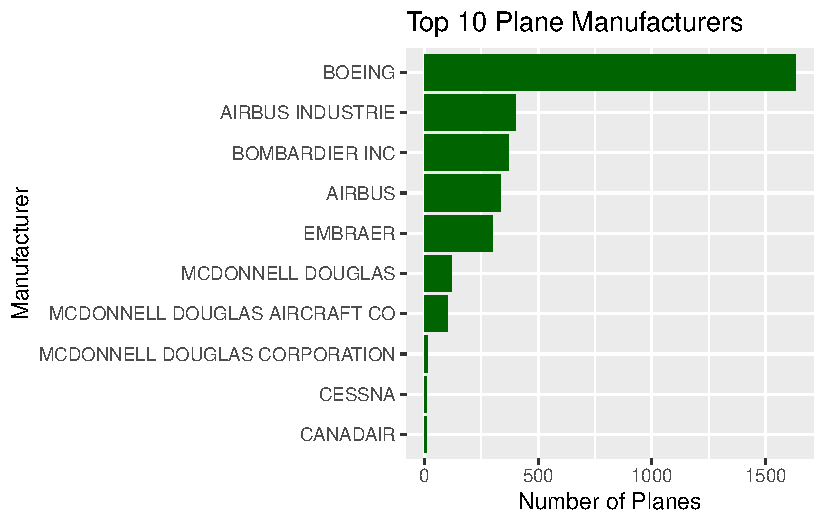
\includegraphics{6-StatistciallySpeaking_files/figure-latex/unnamed-chunk-9-1.pdf}

As we can see from above, Skywest Airlines Inc has the highest
cancellation rate, with Mesa Airlines very closely behind, and a huge
drop off at Endeavor Air Inc.~\#\# Planes Dataset EDA

\subsection{Flights Dataset EDA:}\label{flights-dataset-eda}

\begin{verbatim}
## 
## Missing values per column:
\end{verbatim}

\begin{verbatim}
##           year          month            day       dep_time sched_dep_time 
##              0              0              0           8255              0 
##      dep_delay       arr_time sched_arr_time      arr_delay        carrier 
##           8255           8713              0           9430              0 
##         flight        tailnum         origin           dest       air_time 
##              0           2512              0              0           9430 
##       distance           hour         minute      time_hour 
##              0              0              0              0
\end{verbatim}

\begin{verbatim}
## 
## Column types and structure:
\end{verbatim}

\begin{verbatim}
## Rows: 336,776
## Columns: 19
## $ year           <int> 2013, 2013, 2013, 2013, 2013, 2013, 2013, 2013, 2013, 2~
## $ month          <int> 1, 1, 1, 1, 1, 1, 1, 1, 1, 1, 1, 1, 1, 1, 1, 1, 1, 1, 1~
## $ day            <int> 1, 1, 1, 1, 1, 1, 1, 1, 1, 1, 1, 1, 1, 1, 1, 1, 1, 1, 1~
## $ dep_time       <int> 517, 533, 542, 544, 554, 554, 555, 557, 557, 558, 558, ~
## $ sched_dep_time <int> 515, 529, 540, 545, 600, 558, 600, 600, 600, 600, 600, ~
## $ dep_delay      <dbl> 2, 4, 2, -1, -6, -4, -5, -3, -3, -2, -2, -2, -2, -2, -1~
## $ arr_time       <int> 830, 850, 923, 1004, 812, 740, 913, 709, 838, 753, 849,~
## $ sched_arr_time <int> 819, 830, 850, 1022, 837, 728, 854, 723, 846, 745, 851,~
## $ arr_delay      <dbl> 11, 20, 33, -18, -25, 12, 19, -14, -8, 8, -2, -3, 7, -1~
## $ carrier        <chr> "UA", "UA", "AA", "B6", "DL", "UA", "B6", "EV", "B6", "~
## $ flight         <int> 1545, 1714, 1141, 725, 461, 1696, 507, 5708, 79, 301, 4~
## $ tailnum        <chr> "N14228", "N24211", "N619AA", "N804JB", "N668DN", "N394~
## $ origin         <chr> "EWR", "LGA", "JFK", "JFK", "LGA", "EWR", "EWR", "LGA",~
## $ dest           <chr> "IAH", "IAH", "MIA", "BQN", "ATL", "ORD", "FLL", "IAD",~
## $ air_time       <dbl> 227, 227, 160, 183, 116, 150, 158, 53, 140, 138, 149, 1~
## $ distance       <dbl> 1400, 1416, 1089, 1576, 762, 719, 1065, 229, 944, 733, ~
## $ hour           <dbl> 5, 5, 5, 5, 6, 5, 6, 6, 6, 6, 6, 6, 6, 6, 6, 5, 6, 6, 6~
## $ minute         <dbl> 15, 29, 40, 45, 0, 58, 0, 0, 0, 0, 0, 0, 0, 0, 0, 59, 0~
## $ time_hour      <dttm> 2013-01-01 05:00:00, 2013-01-01 05:00:00, 2013-01-01 0~
## # A tibble: 336,776 x 19
##     year month   day dep_time sched_dep_time dep_delay arr_time sched_arr_time
##    <int> <int> <int>    <int>          <int>     <dbl>    <int>          <int>
##  1  2013     1     1      517            515         2      830            819
##  2  2013     1     1      533            529         4      850            830
##  3  2013     1     1      542            540         2      923            850
##  4  2013     1     1      544            545        -1     1004           1022
##  5  2013     1     1      554            600        -6      812            837
##  6  2013     1     1      554            558        -4      740            728
##  7  2013     1     1      555            600        -5      913            854
##  8  2013     1     1      557            600        -3      709            723
##  9  2013     1     1      557            600        -3      838            846
## 10  2013     1     1      558            600        -2      753            745
## # i 336,766 more rows
## # i 11 more variables: arr_delay <dbl>, carrier <chr>, flight <int>,
## #   tailnum <chr>, origin <chr>, dest <chr>, air_time <dbl>, distance <dbl>,
## #   hour <dbl>, minute <dbl>, time_hour <dttm>
\end{verbatim}

\begin{verbatim}
## 
## First few rows:
\end{verbatim}

\begin{verbatim}
## # A tibble: 6 x 19
##    year month   day dep_time sched_dep_time dep_delay arr_time sched_arr_time
##   <int> <int> <int>    <int>          <int>     <dbl>    <int>          <int>
## 1  2013     1     1      517            515         2      830            819
## 2  2013     1     1      533            529         4      850            830
## 3  2013     1     1      542            540         2      923            850
## 4  2013     1     1      544            545        -1     1004           1022
## 5  2013     1     1      554            600        -6      812            837
## 6  2013     1     1      554            558        -4      740            728
## # i 11 more variables: arr_delay <dbl>, carrier <chr>, flight <int>,
## #   tailnum <chr>, origin <chr>, dest <chr>, air_time <dbl>, distance <dbl>,
## #   hour <dbl>, minute <dbl>, time_hour <dttm>
\end{verbatim}

\begin{verbatim}
## 
## Summary statistics:
\end{verbatim}

\begin{verbatim}
##       year          month             day           dep_time    sched_dep_time
##  Min.   :2013   Min.   : 1.000   Min.   : 1.00   Min.   :   1   Min.   : 106  
##  1st Qu.:2013   1st Qu.: 4.000   1st Qu.: 8.00   1st Qu.: 907   1st Qu.: 906  
##  Median :2013   Median : 7.000   Median :16.00   Median :1401   Median :1359  
##  Mean   :2013   Mean   : 6.549   Mean   :15.71   Mean   :1349   Mean   :1344  
##  3rd Qu.:2013   3rd Qu.:10.000   3rd Qu.:23.00   3rd Qu.:1744   3rd Qu.:1729  
##  Max.   :2013   Max.   :12.000   Max.   :31.00   Max.   :2400   Max.   :2359  
##                                                  NA's   :8255                 
##    dep_delay          arr_time    sched_arr_time   arr_delay       
##  Min.   : -43.00   Min.   :   1   Min.   :   1   Min.   : -86.000  
##  1st Qu.:  -5.00   1st Qu.:1104   1st Qu.:1124   1st Qu.: -17.000  
##  Median :  -2.00   Median :1535   Median :1556   Median :  -5.000  
##  Mean   :  12.64   Mean   :1502   Mean   :1536   Mean   :   6.895  
##  3rd Qu.:  11.00   3rd Qu.:1940   3rd Qu.:1945   3rd Qu.:  14.000  
##  Max.   :1301.00   Max.   :2400   Max.   :2359   Max.   :1272.000  
##  NA's   :8255      NA's   :8713                  NA's   :9430      
##    carrier              flight       tailnum             origin         
##  Length:336776      Min.   :   1   Length:336776      Length:336776     
##  Class :character   1st Qu.: 553   Class :character   Class :character  
##  Mode  :character   Median :1496   Mode  :character   Mode  :character  
##                     Mean   :1972                                        
##                     3rd Qu.:3465                                        
##                     Max.   :8500                                        
##                                                                         
##      dest              air_time        distance         hour      
##  Length:336776      Min.   : 20.0   Min.   :  17   Min.   : 1.00  
##  Class :character   1st Qu.: 82.0   1st Qu.: 502   1st Qu.: 9.00  
##  Mode  :character   Median :129.0   Median : 872   Median :13.00  
##                     Mean   :150.7   Mean   :1040   Mean   :13.18  
##                     3rd Qu.:192.0   3rd Qu.:1389   3rd Qu.:17.00  
##                     Max.   :695.0   Max.   :4983   Max.   :23.00  
##                     NA's   :9430                                  
##      minute        time_hour                     
##  Min.   : 0.00   Min.   :2013-01-01 05:00:00.00  
##  1st Qu.: 8.00   1st Qu.:2013-04-04 13:00:00.00  
##  Median :29.00   Median :2013-07-03 10:00:00.00  
##  Mean   :26.23   Mean   :2013-07-03 05:22:54.64  
##  3rd Qu.:44.00   3rd Qu.:2013-10-01 07:00:00.00  
##  Max.   :59.00   Max.   :2013-12-31 23:00:00.00  
## 
\end{verbatim}

Most of our analysis is based on how other variables and datasets affect
and compare to the flights dataset. We are seeing how the arrival time,
departure delay time, departure time, arrival delay time, and other
variables are affected.

flights that were not canceled ~We will be using these the not\_canceled
data for the rest of the EDA

\begin{Shaded}
\begin{Highlighting}[]
\NormalTok{not\_canceled }\OtherTok{\textless{}{-}} \FunctionTok{filter}\NormalTok{(flights, }\SpecialCharTok{!}\FunctionTok{is.na}\NormalTok{(dep\_delay), }\SpecialCharTok{!}\FunctionTok{is.na}\NormalTok{(arr\_delay))}
\NormalTok{not\_canceled}
\end{Highlighting}
\end{Shaded}

\begin{verbatim}
## # A tibble: 327,346 x 19
##     year month   day dep_time sched_dep_time dep_delay arr_time sched_arr_time
##    <int> <int> <int>    <int>          <int>     <dbl>    <int>          <int>
##  1  2013     1     1      517            515         2      830            819
##  2  2013     1     1      533            529         4      850            830
##  3  2013     1     1      542            540         2      923            850
##  4  2013     1     1      544            545        -1     1004           1022
##  5  2013     1     1      554            600        -6      812            837
##  6  2013     1     1      554            558        -4      740            728
##  7  2013     1     1      555            600        -5      913            854
##  8  2013     1     1      557            600        -3      709            723
##  9  2013     1     1      557            600        -3      838            846
## 10  2013     1     1      558            600        -2      753            745
## # i 327,336 more rows
## # i 11 more variables: arr_delay <dbl>, carrier <chr>, flight <int>,
## #   tailnum <chr>, origin <chr>, dest <chr>, air_time <dbl>, distance <dbl>,
## #   hour <dbl>, minute <dbl>, time_hour <dttm>
\end{verbatim}

Basic delay analysis Distribution and Proportion of delayed flights that
were not canceled

\begin{Shaded}
\begin{Highlighting}[]
\CommentTok{\#histograms}
\FunctionTok{hist}\NormalTok{(not\_canceled}\SpecialCharTok{$}\NormalTok{dep\_delay, }\AttributeTok{breaks=}\DecValTok{100}\NormalTok{, }\AttributeTok{main =} \StringTok{"Departure Delays"}\NormalTok{,}\AttributeTok{xlab =} \StringTok{"Minutes"}\NormalTok{)}
\end{Highlighting}
\end{Shaded}

\includegraphics{6-StatistciallySpeaking_files/figure-latex/unnamed-chunk-12-1.pdf}

\begin{Shaded}
\begin{Highlighting}[]
\FunctionTok{hist}\NormalTok{(not\_canceled}\SpecialCharTok{$}\NormalTok{arr\_delay, }\AttributeTok{breaks=}\DecValTok{100}\NormalTok{, }\AttributeTok{main =}\StringTok{"Arrival Delays"}\NormalTok{, }\AttributeTok{xlab =} \StringTok{"Minutes"}\NormalTok{)}
\end{Highlighting}
\end{Shaded}

\includegraphics{6-StatistciallySpeaking_files/figure-latex/unnamed-chunk-12-2.pdf}

\begin{Shaded}
\begin{Highlighting}[]
\CommentTok{\#proportions}
\FunctionTok{mean}\NormalTok{(not\_canceled}\SpecialCharTok{$}\NormalTok{dep\_delay}\SpecialCharTok{\textgreater{}}\DecValTok{0}\NormalTok{, }\AttributeTok{na.rm=}\ConstantTok{TRUE}\NormalTok{)}
\end{Highlighting}
\end{Shaded}

\begin{verbatim}
## [1] 0.3902446
\end{verbatim}

\begin{Shaded}
\begin{Highlighting}[]
\FunctionTok{mean}\NormalTok{(not\_canceled}\SpecialCharTok{$}\NormalTok{arr\_delay}\SpecialCharTok{\textgreater{}}\DecValTok{0}\NormalTok{, }\AttributeTok{na.rm=}\ConstantTok{TRUE}\NormalTok{)}
\end{Highlighting}
\end{Shaded}

\begin{verbatim}
## [1] 0.4063101
\end{verbatim}

Most of the departure delays do not go over 200 minutes and the arrival
delays have very few delays past 200 minutes.

\paragraph{Delay patterns}\label{delay-patterns}

\begin{Shaded}
\begin{Highlighting}[]
\CommentTok{\#convert time to hours}
\NormalTok{not\_canceled}\SpecialCharTok{$}\NormalTok{dep\_hour }\OtherTok{\textless{}{-}}\FunctionTok{floor}\NormalTok{(not\_canceled}\SpecialCharTok{$}\NormalTok{sched\_dep\_time}\SpecialCharTok{/}\DecValTok{100}\NormalTok{)}
\NormalTok{not\_canceled}\SpecialCharTok{$}\NormalTok{arr\_hour }\OtherTok{\textless{}{-}}\FunctionTok{floor}\NormalTok{(not\_canceled}\SpecialCharTok{$}\NormalTok{sched\_arr\_time}\SpecialCharTok{/}\DecValTok{100}\NormalTok{)}

\CommentTok{\#plot}
\NormalTok{not\_canceled }\SpecialCharTok{|\textgreater{}}
  \FunctionTok{group\_by}\NormalTok{(dep\_hour) }\SpecialCharTok{|\textgreater{}}
  \FunctionTok{summarize}\NormalTok{(}\AttributeTok{mean\_dep\_delay =} \FunctionTok{mean}\NormalTok{(dep\_delay, }\AttributeTok{na.rm=}\ConstantTok{TRUE}\NormalTok{))}\SpecialCharTok{|\textgreater{}}
  \FunctionTok{ggplot}\NormalTok{(}\FunctionTok{aes}\NormalTok{(}\AttributeTok{x=}\NormalTok{dep\_hour, }\AttributeTok{y =}\NormalTok{mean\_dep\_delay))}\SpecialCharTok{+}
  \FunctionTok{geom\_line}\NormalTok{()}\SpecialCharTok{+}
  \FunctionTok{geom\_point}\NormalTok{()}\SpecialCharTok{+}
  \FunctionTok{labs}\NormalTok{(}\AttributeTok{title =} \StringTok{"Average Departure Delay by Hour"}\NormalTok{, }\AttributeTok{x=}\StringTok{"Scheduled Departure"}\NormalTok{, }\AttributeTok{y=}\StringTok{"Minutes"}\NormalTok{)}
\end{Highlighting}
\end{Shaded}

\includegraphics{6-StatistciallySpeaking_files/figure-latex/unnamed-chunk-13-1.pdf}

We can see that many of the delays happen further in the day and peak at
about 18 hours and then it descends from there.

\paragraph{Delays by Airport}\label{delays-by-airport}

\begin{Shaded}
\begin{Highlighting}[]
\NormalTok{not\_canceled }\SpecialCharTok{|\textgreater{}}
  \FunctionTok{group\_by}\NormalTok{(origin)}\SpecialCharTok{|\textgreater{}}
  \FunctionTok{summarize}\NormalTok{(}\AttributeTok{avg\_dep\_delay=} \FunctionTok{mean}\NormalTok{(dep\_delay, }\AttributeTok{na.rm=}\ConstantTok{TRUE}\NormalTok{), }\AttributeTok{avg\_arr\_delay=} \FunctionTok{mean}\NormalTok{(arr\_delay, }\AttributeTok{na.rm=}\ConstantTok{TRUE}\NormalTok{))}
\end{Highlighting}
\end{Shaded}

\begin{verbatim}
## # A tibble: 3 x 3
##   origin avg_dep_delay avg_arr_delay
##   <chr>          <dbl>         <dbl>
## 1 EWR             15.0          9.11
## 2 JFK             12.0          5.55
## 3 LGA             10.3          5.78
\end{verbatim}

EWR has the highest average departure and arrival delay followed by JFK
and then LGA

\subparagraph{Ranking airlines by
delay}\label{ranking-airlines-by-delay}

\begin{Shaded}
\begin{Highlighting}[]
\NormalTok{not\_canceled}\SpecialCharTok{|\textgreater{}}
  \FunctionTok{group\_by}\NormalTok{(carrier)}\SpecialCharTok{|\textgreater{}}
  \FunctionTok{summarize}\NormalTok{(}\AttributeTok{avg\_dep\_delay =} \FunctionTok{mean}\NormalTok{(dep\_delay, }\AttributeTok{na.rn=}\ConstantTok{TRUE}\NormalTok{))}\SpecialCharTok{|\textgreater{}}
  \FunctionTok{arrange}\NormalTok{(}\FunctionTok{desc}\NormalTok{(avg\_dep\_delay))}
\end{Highlighting}
\end{Shaded}

\begin{verbatim}
## # A tibble: 16 x 2
##    carrier avg_dep_delay
##    <chr>           <dbl>
##  1 F9              20.2 
##  2 EV              19.8 
##  3 YV              18.9 
##  4 FL              18.6 
##  5 WN              17.7 
##  6 9E              16.4 
##  7 B6              13.0 
##  8 VX              12.8 
##  9 OO              12.6 
## 10 UA              12.0 
## 11 MQ              10.4 
## 12 DL               9.22
## 13 AA               8.57
## 14 AS               5.83
## 15 HA               4.90
## 16 US               3.74
\end{verbatim}

F9 has the highest average departure delay at 20 hours.

Check to see if the flights that were delayed made up the time in the
air

\begin{Shaded}
\begin{Highlighting}[]
\NormalTok{not\_canceled}\SpecialCharTok{|\textgreater{}}
  \FunctionTok{mutate}\NormalTok{(}\AttributeTok{made\_up\_time =}\NormalTok{ dep\_delay}\SpecialCharTok{{-}}\NormalTok{ arr\_delay)}\SpecialCharTok{|\textgreater{}}
  \FunctionTok{ggplot}\NormalTok{(}\FunctionTok{aes}\NormalTok{(}\AttributeTok{x=}\NormalTok{made\_up\_time))}\SpecialCharTok{+}
  \FunctionTok{geom\_histogram}\NormalTok{(}\AttributeTok{bins=}\DecValTok{100}\NormalTok{)}\SpecialCharTok{+}
  \FunctionTok{labs}\NormalTok{(}\AttributeTok{titel=}\StringTok{"Made up Time in Air"}\NormalTok{, }\AttributeTok{x=} \StringTok{"Minutes Saved"}\NormalTok{, }\AttributeTok{y=}\StringTok{"Count"}\NormalTok{)}
\end{Highlighting}
\end{Shaded}

\includegraphics{6-StatistciallySpeaking_files/figure-latex/unnamed-chunk-16-1.pdf}

We can see that the majority of the flights did not save any minutes on
the arrival delay and actually ended up being delayed more. Some flights
did in fact save minutes but it was less than 50\% of all flights.

\subparagraph{Delays by Month}\label{delays-by-month}

\begin{Shaded}
\begin{Highlighting}[]
\NormalTok{not\_canceled}\SpecialCharTok{|\textgreater{}}
  \FunctionTok{group\_by}\NormalTok{(month)}\SpecialCharTok{|\textgreater{}}
  \FunctionTok{summarize}\NormalTok{(}\AttributeTok{mean\_dep\_delay=}\FunctionTok{mean}\NormalTok{(dep\_delay, }\AttributeTok{na.rm=}\ConstantTok{TRUE}\NormalTok{))}\SpecialCharTok{|\textgreater{}}
  \FunctionTok{ggplot}\NormalTok{(}\FunctionTok{aes}\NormalTok{(}\AttributeTok{x=}\NormalTok{month, }\AttributeTok{y=}\NormalTok{mean\_dep\_delay))}\SpecialCharTok{+}
  \FunctionTok{geom\_line}\NormalTok{()}\SpecialCharTok{+}
  \FunctionTok{geom\_point}\NormalTok{()}\SpecialCharTok{+}
  \FunctionTok{labs}\NormalTok{(}\AttributeTok{title =} \StringTok{"Monthly Departure Delays"}\NormalTok{, }\AttributeTok{x=}\StringTok{"Month"}\NormalTok{, }\AttributeTok{y=}\StringTok{"Time (minutes)"}\NormalTok{)}
\end{Highlighting}
\end{Shaded}

\includegraphics{6-StatistciallySpeaking_files/figure-latex/unnamed-chunk-17-1.pdf}

we see that the majority of flights are delayed from May to mid July,
and there is another peak at December. The months with the shorest
delays are September and October.

\subparagraph{Does distance affect the amount of
delays?}\label{does-distance-affect-the-amount-of-delays}

\begin{Shaded}
\begin{Highlighting}[]
\FunctionTok{ggplot}\NormalTok{(not\_canceled, }\FunctionTok{aes}\NormalTok{(}\AttributeTok{x=}\NormalTok{distance, }\AttributeTok{y=}\NormalTok{dep\_delay))}\SpecialCharTok{+}
  \FunctionTok{geom\_point}\NormalTok{(}\AttributeTok{alpha=}\FloatTok{0.2}\NormalTok{)}\SpecialCharTok{+}
  \FunctionTok{geom\_smooth}\NormalTok{(}\AttributeTok{method =} \StringTok{"lm"}\NormalTok{, }\AttributeTok{se=}\ConstantTok{TRUE}\NormalTok{,}\AttributeTok{color=} \StringTok{"Pink"}\NormalTok{)}\SpecialCharTok{+}
  \FunctionTok{labs}\NormalTok{(}\AttributeTok{title =} \StringTok{"Distance vs Departure Delay"}\NormalTok{, }\AttributeTok{x=}\StringTok{"Distance"}\NormalTok{, }\AttributeTok{y=}\StringTok{"Departure Delay"}\NormalTok{)}
\end{Highlighting}
\end{Shaded}

\begin{verbatim}
## `geom_smooth()` using formula = 'y ~ x'
\end{verbatim}

\includegraphics{6-StatistciallySpeaking_files/figure-latex/unnamed-chunk-18-1.pdf}

We can see that there is not much of an effect of Distance on Departure
delay.

\subparagraph{Flights traveled the longest by
distance}\label{flights-traveled-the-longest-by-distance}

\begin{Shaded}
\begin{Highlighting}[]
\NormalTok{longest\_Distance }\OtherTok{\textless{}{-}}\NormalTok{ not\_canceled }\SpecialCharTok{|\textgreater{}}
  \FunctionTok{arrange}\NormalTok{(}\FunctionTok{desc}\NormalTok{(distance)) }\SpecialCharTok{|\textgreater{}}
\NormalTok{  dplyr}\SpecialCharTok{::}\FunctionTok{select}\NormalTok{(carrier, origin, dest)}
\NormalTok{longest\_Distance}
\end{Highlighting}
\end{Shaded}

\begin{verbatim}
## # A tibble: 327,346 x 3
##    carrier origin dest 
##    <chr>   <chr>  <chr>
##  1 HA      JFK    HNL  
##  2 HA      JFK    HNL  
##  3 HA      JFK    HNL  
##  4 HA      JFK    HNL  
##  5 HA      JFK    HNL  
##  6 HA      JFK    HNL  
##  7 HA      JFK    HNL  
##  8 HA      JFK    HNL  
##  9 HA      JFK    HNL  
## 10 HA      JFK    HNL  
## # i 327,336 more rows
\end{verbatim}

We see that HA is the carrier with the longest flights and they all
start at JFK airport and land at HNL.

\subparagraph{arrival delays per
carrier}\label{arrival-delays-per-carrier}

\begin{Shaded}
\begin{Highlighting}[]
\NormalTok{carrier\_Dest}\OtherTok{\textless{}{-}}\NormalTok{not\_canceled }\SpecialCharTok{|\textgreater{}}
  \FunctionTok{group\_by}\NormalTok{(carrier, dest) }\SpecialCharTok{|\textgreater{}}
  \FunctionTok{summarize}\NormalTok{(}\AttributeTok{avg\_arr\_Delay =} \FunctionTok{mean}\NormalTok{(arr\_delay, }\AttributeTok{na.rm=} \ConstantTok{TRUE}\NormalTok{), }\AttributeTok{.group=} \StringTok{"drop"}\NormalTok{)}
\end{Highlighting}
\end{Shaded}

\begin{verbatim}
## `summarise()` has grouped output by 'carrier'. You can override using the
## `.groups` argument.
\end{verbatim}

\begin{Shaded}
\begin{Highlighting}[]
  \FunctionTok{ggplot}\NormalTok{(carrier\_Dest, }\FunctionTok{aes}\NormalTok{(}\AttributeTok{x =} \FunctionTok{reorder}\NormalTok{(carrier, avg\_arr\_Delay, median), }\AttributeTok{y=}\NormalTok{ avg\_arr\_Delay))}\SpecialCharTok{+}
  \FunctionTok{geom\_boxplot}\NormalTok{()}\SpecialCharTok{+}
  \FunctionTok{coord\_flip}\NormalTok{()}\SpecialCharTok{+}
  \FunctionTok{labs}\NormalTok{(}\AttributeTok{title =} \StringTok{"Average Arrival Delay by Carrier"}\NormalTok{,}\AttributeTok{x =} \StringTok{"Carrier"}\NormalTok{, }\AttributeTok{y=} \StringTok{"Average Arrival Delay (minutes)"}\NormalTok{)}\SpecialCharTok{+}
  \FunctionTok{theme\_minimal}\NormalTok{()}
\end{Highlighting}
\end{Shaded}

\includegraphics{6-StatistciallySpeaking_files/figure-latex/unnamed-chunk-20-1.pdf}

\subsection{Weather Dataset EDA}\label{weather-dataset-eda}

\begin{verbatim}
## 
## Missing values per column:
\end{verbatim}

\begin{verbatim}
##     origin       year      month        day       hour       temp       dewp 
##          0          0          0          0          0          1          1 
##      humid   wind_dir wind_speed  wind_gust     precip   pressure      visib 
##          1        460          4      20778          0       2729          0 
##  time_hour 
##          0
\end{verbatim}

\begin{verbatim}
## 
## Column types and structure:
\end{verbatim}

\begin{verbatim}
## Rows: 26,115
## Columns: 15
## $ origin     <chr> "EWR", "EWR", "EWR", "EWR", "EWR", "EWR", "EWR", "EWR", "EW~
## $ year       <int> 2013, 2013, 2013, 2013, 2013, 2013, 2013, 2013, 2013, 2013,~
## $ month      <int> 1, 1, 1, 1, 1, 1, 1, 1, 1, 1, 1, 1, 1, 1, 1, 1, 1, 1, 1, 1,~
## $ day        <int> 1, 1, 1, 1, 1, 1, 1, 1, 1, 1, 1, 1, 1, 1, 1, 1, 1, 1, 1, 1,~
## $ hour       <int> 1, 2, 3, 4, 5, 6, 7, 8, 9, 10, 11, 13, 14, 15, 16, 17, 18, ~
## $ temp       <dbl> 39.02, 39.02, 39.02, 39.92, 39.02, 37.94, 39.02, 39.92, 39.~
## $ dewp       <dbl> 26.06, 26.96, 28.04, 28.04, 28.04, 28.04, 28.04, 28.04, 28.~
## $ humid      <dbl> 59.37, 61.63, 64.43, 62.21, 64.43, 67.21, 64.43, 62.21, 62.~
## $ wind_dir   <dbl> 270, 250, 240, 250, 260, 240, 240, 250, 260, 260, 260, 330,~
## $ wind_speed <dbl> 10.35702, 8.05546, 11.50780, 12.65858, 12.65858, 11.50780, ~
## $ wind_gust  <dbl> NA, NA, NA, NA, NA, NA, NA, NA, NA, NA, NA, NA, NA, NA, 20.~
## $ precip     <dbl> 0, 0, 0, 0, 0, 0, 0, 0, 0, 0, 0, 0, 0, 0, 0, 0, 0, 0, 0, 0,~
## $ pressure   <dbl> 1012.0, 1012.3, 1012.5, 1012.2, 1011.9, 1012.4, 1012.2, 101~
## $ visib      <dbl> 10, 10, 10, 10, 10, 10, 10, 10, 10, 10, 10, 10, 10, 10, 10,~
## $ time_hour  <dttm> 2013-01-01 01:00:00, 2013-01-01 02:00:00, 2013-01-01 03:00~
## # A tibble: 26,115 x 15
##    origin  year month   day  hour  temp  dewp humid wind_dir wind_speed
##    <chr>  <int> <int> <int> <int> <dbl> <dbl> <dbl>    <dbl>      <dbl>
##  1 EWR     2013     1     1     1  39.0  26.1  59.4      270      10.4 
##  2 EWR     2013     1     1     2  39.0  27.0  61.6      250       8.06
##  3 EWR     2013     1     1     3  39.0  28.0  64.4      240      11.5 
##  4 EWR     2013     1     1     4  39.9  28.0  62.2      250      12.7 
##  5 EWR     2013     1     1     5  39.0  28.0  64.4      260      12.7 
##  6 EWR     2013     1     1     6  37.9  28.0  67.2      240      11.5 
##  7 EWR     2013     1     1     7  39.0  28.0  64.4      240      15.0 
##  8 EWR     2013     1     1     8  39.9  28.0  62.2      250      10.4 
##  9 EWR     2013     1     1     9  39.9  28.0  62.2      260      15.0 
## 10 EWR     2013     1     1    10  41    28.0  59.6      260      13.8 
## # i 26,105 more rows
## # i 5 more variables: wind_gust <dbl>, precip <dbl>, pressure <dbl>,
## #   visib <dbl>, time_hour <dttm>
\end{verbatim}

\begin{verbatim}
## 
## First few rows:
\end{verbatim}

\begin{verbatim}
## # A tibble: 6 x 15
##   origin  year month   day  hour  temp  dewp humid wind_dir wind_speed wind_gust
##   <chr>  <int> <int> <int> <int> <dbl> <dbl> <dbl>    <dbl>      <dbl>     <dbl>
## 1 EWR     2013     1     1     1  39.0  26.1  59.4      270      10.4         NA
## 2 EWR     2013     1     1     2  39.0  27.0  61.6      250       8.06        NA
## 3 EWR     2013     1     1     3  39.0  28.0  64.4      240      11.5         NA
## 4 EWR     2013     1     1     4  39.9  28.0  62.2      250      12.7         NA
## 5 EWR     2013     1     1     5  39.0  28.0  64.4      260      12.7         NA
## 6 EWR     2013     1     1     6  37.9  28.0  67.2      240      11.5         NA
## # i 4 more variables: precip <dbl>, pressure <dbl>, visib <dbl>,
## #   time_hour <dttm>
\end{verbatim}

\begin{verbatim}
## 
## Summary statistics:
\end{verbatim}

\begin{verbatim}
##     origin               year          month             day       
##  Length:26115       Min.   :2013   Min.   : 1.000   Min.   : 1.00  
##  Class :character   1st Qu.:2013   1st Qu.: 4.000   1st Qu.: 8.00  
##  Mode  :character   Median :2013   Median : 7.000   Median :16.00  
##                     Mean   :2013   Mean   : 6.504   Mean   :15.68  
##                     3rd Qu.:2013   3rd Qu.: 9.000   3rd Qu.:23.00  
##                     Max.   :2013   Max.   :12.000   Max.   :31.00  
##                                                                    
##       hour            temp             dewp           humid       
##  Min.   : 0.00   Min.   : 10.94   Min.   :-9.94   Min.   : 12.74  
##  1st Qu.: 6.00   1st Qu.: 39.92   1st Qu.:26.06   1st Qu.: 47.05  
##  Median :11.00   Median : 55.40   Median :42.08   Median : 61.79  
##  Mean   :11.49   Mean   : 55.26   Mean   :41.44   Mean   : 62.53  
##  3rd Qu.:17.00   3rd Qu.: 69.98   3rd Qu.:57.92   3rd Qu.: 78.79  
##  Max.   :23.00   Max.   :100.04   Max.   :78.08   Max.   :100.00  
##                  NA's   :1        NA's   :1       NA's   :1       
##     wind_dir       wind_speed         wind_gust         precip        
##  Min.   :  0.0   Min.   :   0.000   Min.   :16.11   Min.   :0.000000  
##  1st Qu.:120.0   1st Qu.:   6.905   1st Qu.:20.71   1st Qu.:0.000000  
##  Median :220.0   Median :  10.357   Median :24.17   Median :0.000000  
##  Mean   :199.8   Mean   :  10.518   Mean   :25.49   Mean   :0.004469  
##  3rd Qu.:290.0   3rd Qu.:  13.809   3rd Qu.:28.77   3rd Qu.:0.000000  
##  Max.   :360.0   Max.   :1048.361   Max.   :66.75   Max.   :1.210000  
##  NA's   :460     NA's   :4          NA's   :20778                     
##     pressure          visib          time_hour                    
##  Min.   : 983.8   Min.   : 0.000   Min.   :2013-01-01 01:00:00.0  
##  1st Qu.:1012.9   1st Qu.:10.000   1st Qu.:2013-04-01 21:30:00.0  
##  Median :1017.6   Median :10.000   Median :2013-07-01 14:00:00.0  
##  Mean   :1017.9   Mean   : 9.255   Mean   :2013-07-01 18:26:37.7  
##  3rd Qu.:1023.0   3rd Qu.:10.000   3rd Qu.:2013-09-30 13:00:00.0  
##  Max.   :1042.1   Max.   :10.000   Max.   :2013-12-30 18:00:00.0  
##  NA's   :2729
\end{verbatim}

\begin{Shaded}
\begin{Highlighting}[]
\CommentTok{\# Related Questions from our Proposal:}
\CommentTok{\# {-}{-}{-} How do weather conditions affect flight delays? }
\CommentTok{\# {-}{-}{-} How do environmental factors like humidity, visibility, and wind affect flight delays? }
\CommentTok{\# {-}{-}{-} What impact does precipitation have on specific airports and weather{-}related delays? }


\CommentTok{\# Average Temperature by Month}
\CommentTok{\# {-}{-}{-} We can see that the average temperature ranges from about 70{-}80º in the summer, and 35{-}40º in the winter. }
\CommentTok{\# {-}{-}{-} When answering our research questions, we can see if there is a correlation between summer/winter weather and flight delays.}

\NormalTok{monthlyavgtemp }\OtherTok{\textless{}{-}}\NormalTok{ weather }\SpecialCharTok{\%\textgreater{}\%}
  \FunctionTok{group\_by}\NormalTok{(month) }\SpecialCharTok{\%\textgreater{}\%}
  \FunctionTok{summarise}\NormalTok{(}\AttributeTok{monthlyavgtemp =} \FunctionTok{mean}\NormalTok{(temp, }\AttributeTok{na.rm =} \ConstantTok{TRUE}\NormalTok{))}

\FunctionTok{ggplot}\NormalTok{(}\AttributeTok{data =}\NormalTok{ monthlyavgtemp,}
       \FunctionTok{aes}\NormalTok{(}\AttributeTok{x =} \FunctionTok{factor}\NormalTok{(month), }\AttributeTok{y =}\NormalTok{ monthlyavgtemp)) }\SpecialCharTok{+}
  \FunctionTok{geom\_col}\NormalTok{(}\AttributeTok{color =} \StringTok{"skyblue"}\NormalTok{, }\AttributeTok{fill =} \StringTok{"lightskyblue1"}\NormalTok{) }\SpecialCharTok{+} 
  \FunctionTok{labs}\NormalTok{(}\AttributeTok{title =} \StringTok{"Average Temperature by Month"}\NormalTok{,}
       \AttributeTok{x =} \StringTok{"Month"}\NormalTok{,}
       \AttributeTok{y =} \StringTok{"Average Temperature (Fº)"}\NormalTok{) }\SpecialCharTok{+}
  \FunctionTok{theme\_minimal}\NormalTok{()}
\end{Highlighting}
\end{Shaded}

\includegraphics{6-StatistciallySpeaking_files/figure-latex/unnamed-chunk-22-1.pdf}

\begin{Shaded}
\begin{Highlighting}[]
\CommentTok{\# Average Visibility by Month}
\CommentTok{\# {-}{-}{-} The average visibility does not greatly vary by month looking at the average value. However, we can see that there is slightly less visiblity in winter months.}
\CommentTok{\# {-}{-}{-} Looking at the boxplots, we can see that there are a lot of outliers. Removing these outliers and focusing on visib \textless{} 10 shows us a better distribution of visiblity.}
\CommentTok{\# {-}{-}{-} When answering our research questions, we can compare the average visibility during flight delays vs average visibility without flight       delays to further explore the role of visibility in flight delays. }

\NormalTok{monthlyavgvisib }\OtherTok{\textless{}{-}}\NormalTok{ weather }\SpecialCharTok{\%\textgreater{}\%}
  \FunctionTok{group\_by}\NormalTok{(month) }\SpecialCharTok{\%\textgreater{}\%}
  \FunctionTok{summarise}\NormalTok{(}\AttributeTok{monthlyavgvisib =} \FunctionTok{mean}\NormalTok{(visib, }\AttributeTok{na.rm =} \ConstantTok{TRUE}\NormalTok{))}

\FunctionTok{ggplot}\NormalTok{(}\AttributeTok{data =}\NormalTok{ monthlyavgvisib) }\SpecialCharTok{+}
    \FunctionTok{geom\_col}\NormalTok{(}\FunctionTok{aes}\NormalTok{(}\AttributeTok{x =} \FunctionTok{factor}\NormalTok{(month), }\AttributeTok{y =}\NormalTok{ monthlyavgvisib),}
                   \AttributeTok{color =} \StringTok{"orchid4"}\NormalTok{, }\AttributeTok{fill =} \StringTok{"plum"}\NormalTok{) }\SpecialCharTok{+} 
  \FunctionTok{labs}\NormalTok{(}\AttributeTok{title =} \StringTok{"Average Visibility by Month"}\NormalTok{,}
       \AttributeTok{x =} \StringTok{"Month"}\NormalTok{,}
       \AttributeTok{y =} \StringTok{"Average Visibility"}\NormalTok{) }\SpecialCharTok{+}
  \FunctionTok{theme\_minimal}\NormalTok{()}
\end{Highlighting}
\end{Shaded}

\includegraphics{6-StatistciallySpeaking_files/figure-latex/unnamed-chunk-22-2.pdf}

\begin{Shaded}
\begin{Highlighting}[]
\FunctionTok{ggplot}\NormalTok{(weather, }\FunctionTok{aes}\NormalTok{(}\AttributeTok{x =} \FunctionTok{factor}\NormalTok{(month), }\AttributeTok{y =}\NormalTok{ visib)) }\SpecialCharTok{+}
  \FunctionTok{geom\_boxplot}\NormalTok{(}\AttributeTok{fill =} \StringTok{"plum"}\NormalTok{, }\AttributeTok{color =} \StringTok{"orchid4"}\NormalTok{) }\SpecialCharTok{+}
  \FunctionTok{labs}\NormalTok{(}\AttributeTok{title =} \StringTok{"Distribution of Visibility by Month"}\NormalTok{,}
       \AttributeTok{x =} \StringTok{"Month"}\NormalTok{,}
       \AttributeTok{y =} \StringTok{"Visibility"}\NormalTok{) }\SpecialCharTok{+}
  \FunctionTok{coord\_flip}\NormalTok{() }\SpecialCharTok{+}
  \FunctionTok{theme\_minimal}\NormalTok{()}
\end{Highlighting}
\end{Shaded}

\includegraphics{6-StatistciallySpeaking_files/figure-latex/unnamed-chunk-22-3.pdf}

\begin{Shaded}
\begin{Highlighting}[]
\FunctionTok{ggplot}\NormalTok{(}\FunctionTok{filter}\NormalTok{(weather, visib }\SpecialCharTok{\textless{}} \DecValTok{10}\NormalTok{), }\FunctionTok{aes}\NormalTok{(}\AttributeTok{x =} \FunctionTok{factor}\NormalTok{(month), }\AttributeTok{y =}\NormalTok{ visib)) }\SpecialCharTok{+}
  \FunctionTok{geom\_boxplot}\NormalTok{(}\AttributeTok{fill =} \StringTok{"plum"}\NormalTok{, }\AttributeTok{color =} \StringTok{"orchid4"}\NormalTok{) }\SpecialCharTok{+}
  \FunctionTok{labs}\NormalTok{(}\AttributeTok{title =} \StringTok{"Distribution of Visibility \textless{} 10 by Month"}\NormalTok{,}
       \AttributeTok{x =} \StringTok{"Month"}\NormalTok{,}
       \AttributeTok{y =} \StringTok{"Visibility"}\NormalTok{) }\SpecialCharTok{+}
  \FunctionTok{coord\_flip}\NormalTok{() }\SpecialCharTok{+}
  \FunctionTok{theme\_minimal}\NormalTok{()}
\end{Highlighting}
\end{Shaded}

\includegraphics{6-StatistciallySpeaking_files/figure-latex/unnamed-chunk-22-4.pdf}

\begin{Shaded}
\begin{Highlighting}[]
\CommentTok{\# Distribution of Humidity by Month}
\CommentTok{\# {-}{-}{-} The distribution of humidity varies by month, but there does not seem to be significant differences.}
\CommentTok{\# {-}{-}{-} We can further explore the role of humidity by comparing it to other weather variables and flight delays.}

\FunctionTok{ggplot}\NormalTok{(weather, }\FunctionTok{aes}\NormalTok{(}\AttributeTok{x =} \FunctionTok{factor}\NormalTok{(month), }\AttributeTok{y =}\NormalTok{ humid)) }\SpecialCharTok{+}
  \FunctionTok{geom\_boxplot}\NormalTok{(}\AttributeTok{fill =} \StringTok{"darkseagreen2"}\NormalTok{, }\AttributeTok{color =} \StringTok{"darkgreen"}\NormalTok{) }\SpecialCharTok{+}
  \FunctionTok{labs}\NormalTok{(}\AttributeTok{title =} \StringTok{"Distribution of Humidity by Month (With Outliers)"}\NormalTok{,}
       \AttributeTok{x =} \StringTok{"Month"}\NormalTok{,}
       \AttributeTok{y =} \StringTok{"Humidity"}\NormalTok{) }\SpecialCharTok{+}
  \FunctionTok{coord\_flip}\NormalTok{() }\SpecialCharTok{+}
  \FunctionTok{theme\_minimal}\NormalTok{()}
\end{Highlighting}
\end{Shaded}

\begin{verbatim}
## Warning: Removed 1 row containing non-finite outside the scale range
## (`stat_boxplot()`).
\end{verbatim}

\includegraphics{6-StatistciallySpeaking_files/figure-latex/unnamed-chunk-22-5.pdf}

\begin{Shaded}
\begin{Highlighting}[]
\CommentTok{\# Precipitation by Month}
\CommentTok{\# {-}{-}{-} The average precipitation for each month varies greatly. We can see that spring months have the greatest average precipitation.}
\CommentTok{\# {-}{-}{-} When answering our research question, we can see if greater precipitation correlates to flight delays. }

\NormalTok{monthlyprecip }\OtherTok{\textless{}{-}}\NormalTok{ weather }\SpecialCharTok{\%\textgreater{}\%}
  \FunctionTok{group\_by}\NormalTok{(month) }\SpecialCharTok{\%\textgreater{}\%}
  \FunctionTok{summarise}\NormalTok{(}\AttributeTok{avgmonthlyprecip =} \FunctionTok{mean}\NormalTok{(precip, }\AttributeTok{na.rm =} \ConstantTok{TRUE}\NormalTok{))}

\FunctionTok{ggplot}\NormalTok{(monthlyprecip, }\FunctionTok{aes}\NormalTok{(}\AttributeTok{x =}\NormalTok{ month, }\AttributeTok{y =}\NormalTok{ avgmonthlyprecip)) }\SpecialCharTok{+}
  \FunctionTok{geom\_line}\NormalTok{(}\AttributeTok{color =} \StringTok{"palevioletred2"}\NormalTok{) }\SpecialCharTok{+}
  \FunctionTok{geom\_point}\NormalTok{(}\AttributeTok{color =} \StringTok{"palevioletred4"}\NormalTok{) }\SpecialCharTok{+}
  \FunctionTok{labs}\NormalTok{(}\AttributeTok{title =} \StringTok{"Average Monthly Precipitation"}\NormalTok{,}
       \AttributeTok{x =} \StringTok{"Month"}\NormalTok{,}
       \AttributeTok{y =} \StringTok{"Average Precipitation"}\NormalTok{) }\SpecialCharTok{+}
  \FunctionTok{scale\_x\_continuous}\NormalTok{(}\AttributeTok{breaks =} \DecValTok{1}\SpecialCharTok{:}\DecValTok{12}\NormalTok{) }\SpecialCharTok{+}
  \FunctionTok{theme\_minimal}\NormalTok{()}
\end{Highlighting}
\end{Shaded}

\includegraphics{6-StatistciallySpeaking_files/figure-latex/unnamed-chunk-22-6.pdf}

\begin{Shaded}
\begin{Highlighting}[]
\CommentTok{\# Correlation Between Variables}
\CommentTok{\# {-}{-}{-} We can explore the correlation between different weather variables and see how they may work together to impact flight delays.}

\FunctionTok{cor}\NormalTok{(weather}\SpecialCharTok{$}\NormalTok{precip, weather}\SpecialCharTok{$}\NormalTok{visib, }\AttributeTok{use =} \StringTok{"complete.obs"}\NormalTok{)}
\end{Highlighting}
\end{Shaded}

\begin{verbatim}
## [1] -0.3199118
\end{verbatim}

\begin{Shaded}
\begin{Highlighting}[]
\FunctionTok{cor}\NormalTok{(weather}\SpecialCharTok{$}\NormalTok{humid, weather}\SpecialCharTok{$}\NormalTok{visib, }\AttributeTok{use =} \StringTok{"complete.obs"}\NormalTok{)}
\end{Highlighting}
\end{Shaded}

\begin{verbatim}
## [1] -0.5167424
\end{verbatim}

\newpage

\section{Analysis Approach Plan}\label{analysis-approach-plan}

\textbf{Assumptions:} All variables are independent

The process of analysis will involve data cleaning after forming our
question, basic exploration of the data, comparison of certain datasets
with other datasets, visualization of the data, and an interpretation of
the data/results. Cleaning of the data will deal with tasks like
handling empty cells/columns and NA values. When it comes to exploratory
data analysis, we plan on using tools such as histograms and boxplots to
gain an understanding of the data and identify patterns and
relationships. The statistical analysis that we plan on performing with
the data will most likely involve making comparisons between groups to
compare airlines, times, and other metrics to make our overall claim.
For example, we might be comparing trends in time performance by weeks
or month between different airlines to gain a better understanding of
how differences in airlines affect delays. In terms of data
visualization, we will most likely be using line graphs for trends over
time when it comes to comparing flight time under different variables
and heatmaps/scatterplots for flight delays to help communicate our
findings. Finally, interpretation of the data will involve us answering
the proposed question by summarizing our statistics/findings as well as
through the presentation of graphical evidence.

\section{Analysis:}\label{analysis}

\subsubsection{Question 1: How do weather conditions affect flight
delays?}\label{question-1-how-do-weather-conditions-affect-flight-delays}

\subsubsection{1. Are specific weather variables (e.g., precipitation,
temperature, humidity) correlated with arrival
delays?}\label{are-specific-weather-variables-e.g.-precipitation-temperature-humidity-correlated-with-arrival-delays}

\begin{Shaded}
\begin{Highlighting}[]
\FunctionTok{head}\NormalTok{(weather)}
\end{Highlighting}
\end{Shaded}

\begin{verbatim}
## # A tibble: 6 x 15
##   origin  year month   day  hour  temp  dewp humid wind_dir wind_speed wind_gust
##   <chr>  <int> <int> <int> <int> <dbl> <dbl> <dbl>    <dbl>      <dbl>     <dbl>
## 1 EWR     2013     1     1     1  39.0  26.1  59.4      270      10.4         NA
## 2 EWR     2013     1     1     2  39.0  27.0  61.6      250       8.06        NA
## 3 EWR     2013     1     1     3  39.0  28.0  64.4      240      11.5         NA
## 4 EWR     2013     1     1     4  39.9  28.0  62.2      250      12.7         NA
## 5 EWR     2013     1     1     5  39.0  28.0  64.4      260      12.7         NA
## 6 EWR     2013     1     1     6  37.9  28.0  67.2      240      11.5         NA
## # i 4 more variables: precip <dbl>, pressure <dbl>, visib <dbl>,
## #   time_hour <dttm>
\end{verbatim}

\begin{Shaded}
\begin{Highlighting}[]
\FunctionTok{head}\NormalTok{(flights)}
\end{Highlighting}
\end{Shaded}

\begin{verbatim}
## # A tibble: 6 x 19
##    year month   day dep_time sched_dep_time dep_delay arr_time sched_arr_time
##   <int> <int> <int>    <int>          <int>     <dbl>    <int>          <int>
## 1  2013     1     1      517            515         2      830            819
## 2  2013     1     1      533            529         4      850            830
## 3  2013     1     1      542            540         2      923            850
## 4  2013     1     1      544            545        -1     1004           1022
## 5  2013     1     1      554            600        -6      812            837
## 6  2013     1     1      554            558        -4      740            728
## # i 11 more variables: arr_delay <dbl>, carrier <chr>, flight <int>,
## #   tailnum <chr>, origin <chr>, dest <chr>, air_time <dbl>, distance <dbl>,
## #   hour <dbl>, minute <dbl>, time_hour <dttm>
\end{verbatim}

\begin{Shaded}
\begin{Highlighting}[]
\NormalTok{not\_canceled }\OtherTok{\textless{}{-}} \FunctionTok{filter}\NormalTok{(flights, }\SpecialCharTok{!}\FunctionTok{is.na}\NormalTok{(dep\_delay), }\SpecialCharTok{!}\FunctionTok{is.na}\NormalTok{(arr\_delay))}
\FunctionTok{head}\NormalTok{(not\_canceled)}
\end{Highlighting}
\end{Shaded}

\begin{verbatim}
## # A tibble: 6 x 19
##    year month   day dep_time sched_dep_time dep_delay arr_time sched_arr_time
##   <int> <int> <int>    <int>          <int>     <dbl>    <int>          <int>
## 1  2013     1     1      517            515         2      830            819
## 2  2013     1     1      533            529         4      850            830
## 3  2013     1     1      542            540         2      923            850
## 4  2013     1     1      544            545        -1     1004           1022
## 5  2013     1     1      554            600        -6      812            837
## 6  2013     1     1      554            558        -4      740            728
## # i 11 more variables: arr_delay <dbl>, carrier <chr>, flight <int>,
## #   tailnum <chr>, origin <chr>, dest <chr>, air_time <dbl>, distance <dbl>,
## #   hour <dbl>, minute <dbl>, time_hour <dttm>
\end{verbatim}

join columns of weather and uncancelled flights

\begin{Shaded}
\begin{Highlighting}[]
\NormalTok{flights\_weather }\OtherTok{\textless{}{-}} \FunctionTok{left\_join}\NormalTok{(not\_canceled, weather, }\AttributeTok{by =} \FunctionTok{c}\NormalTok{(}\StringTok{"year"}\NormalTok{, }\StringTok{"month"}\NormalTok{, }\StringTok{"day"}\NormalTok{, }\StringTok{"hour"}\NormalTok{, }\StringTok{"origin"}\NormalTok{))}

\NormalTok{flights\_weather }\OtherTok{\textless{}{-}}\NormalTok{ flights\_weather }\SpecialCharTok{|\textgreater{}}
  \FunctionTok{filter}\NormalTok{(}\SpecialCharTok{!}\FunctionTok{is.na}\NormalTok{(dep\_delay))}
\NormalTok{flights\_weather}
\end{Highlighting}
\end{Shaded}

\begin{verbatim}
## # A tibble: 327,346 x 29
##     year month   day dep_time sched_dep_time dep_delay arr_time sched_arr_time
##    <int> <int> <int>    <int>          <int>     <dbl>    <int>          <int>
##  1  2013     1     1      517            515         2      830            819
##  2  2013     1     1      533            529         4      850            830
##  3  2013     1     1      542            540         2      923            850
##  4  2013     1     1      544            545        -1     1004           1022
##  5  2013     1     1      554            600        -6      812            837
##  6  2013     1     1      554            558        -4      740            728
##  7  2013     1     1      555            600        -5      913            854
##  8  2013     1     1      557            600        -3      709            723
##  9  2013     1     1      557            600        -3      838            846
## 10  2013     1     1      558            600        -2      753            745
## # i 327,336 more rows
## # i 21 more variables: arr_delay <dbl>, carrier <chr>, flight <int>,
## #   tailnum <chr>, origin <chr>, dest <chr>, air_time <dbl>, distance <dbl>,
## #   hour <dbl>, minute <dbl>, time_hour.x <dttm>, temp <dbl>, dewp <dbl>,
## #   humid <dbl>, wind_dir <dbl>, wind_speed <dbl>, wind_gust <dbl>,
## #   precip <dbl>, pressure <dbl>, visib <dbl>, time_hour.y <dttm>
\end{verbatim}

Temperature by month and departure delays

\begin{Shaded}
\begin{Highlighting}[]
\CommentTok{\#mutate to month }
\NormalTok{f\_w\_by\_month }\OtherTok{\textless{}{-}}\NormalTok{ flights\_weather }\SpecialCharTok{|\textgreater{}}
  \FunctionTok{mutate}\NormalTok{(}\AttributeTok{month =} \FunctionTok{factor}\NormalTok{(month, }\AttributeTok{levels =} \DecValTok{1}\SpecialCharTok{:}\DecValTok{12}\NormalTok{, }\AttributeTok{labels =}\NormalTok{ month.name))}

\FunctionTok{ggplot}\NormalTok{(f\_w\_by\_month, }\FunctionTok{aes}\NormalTok{(}\AttributeTok{x =}\NormalTok{ temp, }\AttributeTok{y =}\NormalTok{ dep\_delay)) }\SpecialCharTok{+} 
  \FunctionTok{geom\_point}\NormalTok{() }\SpecialCharTok{+}
  \FunctionTok{facet\_wrap}\NormalTok{(}\SpecialCharTok{\textasciitilde{}}\NormalTok{ month, }\AttributeTok{ncol =} \DecValTok{3}\NormalTok{)}
\end{Highlighting}
\end{Shaded}

\begin{verbatim}
## Warning: Removed 1544 rows containing missing values or values outside the scale range
## (`geom_point()`).
\end{verbatim}

\includegraphics{6-StatistciallySpeaking_files/figure-latex/unnamed-chunk-25-1.pdf}

\begin{Shaded}
\begin{Highlighting}[]
\FunctionTok{ggplot}\NormalTok{(f\_w\_by\_month, }\FunctionTok{aes}\NormalTok{(}\AttributeTok{x =}\NormalTok{ temp, }\AttributeTok{y =}\NormalTok{ dep\_delay)) }\SpecialCharTok{+}
  \FunctionTok{geom\_bar}\NormalTok{(}\AttributeTok{stat =} \StringTok{"identity"}\NormalTok{)}
\end{Highlighting}
\end{Shaded}

\begin{verbatim}
## Warning: Removed 1544 rows containing missing values or values outside the scale range
## (`geom_bar()`).
\end{verbatim}

\includegraphics{6-StatistciallySpeaking_files/figure-latex/unnamed-chunk-25-2.pdf}

Humidity by month and departure delays

\begin{Shaded}
\begin{Highlighting}[]
\FunctionTok{ggplot}\NormalTok{(f\_w\_by\_month, }\FunctionTok{aes}\NormalTok{(}\AttributeTok{x =}\NormalTok{ humid, }\AttributeTok{y =}\NormalTok{ dep\_delay)) }\SpecialCharTok{+} 
  \FunctionTok{geom\_point}\NormalTok{() }\SpecialCharTok{+}
  \FunctionTok{facet\_wrap}\NormalTok{(}\SpecialCharTok{\textasciitilde{}}\NormalTok{ month, }\AttributeTok{ncol =} \DecValTok{3}\NormalTok{)}
\end{Highlighting}
\end{Shaded}

\begin{verbatim}
## Warning: Removed 1544 rows containing missing values or values outside the scale range
## (`geom_point()`).
\end{verbatim}

\includegraphics{6-StatistciallySpeaking_files/figure-latex/unnamed-chunk-26-1.pdf}

\begin{Shaded}
\begin{Highlighting}[]
\FunctionTok{ggplot}\NormalTok{(f\_w\_by\_month, }\FunctionTok{aes}\NormalTok{(}\AttributeTok{x =}\NormalTok{ humid, }\AttributeTok{y =}\NormalTok{ dep\_delay)) }\SpecialCharTok{+}
  \FunctionTok{geom\_bar}\NormalTok{(}\AttributeTok{stat =} \StringTok{"identity"}\NormalTok{)}
\end{Highlighting}
\end{Shaded}

\begin{verbatim}
## Warning: Removed 1544 rows containing missing values or values outside the scale range
## (`geom_bar()`).
\end{verbatim}

\includegraphics{6-StatistciallySpeaking_files/figure-latex/unnamed-chunk-26-2.pdf}

Precipitation by month and departure delays

\begin{Shaded}
\begin{Highlighting}[]
\FunctionTok{ggplot}\NormalTok{(f\_w\_by\_month, }\FunctionTok{aes}\NormalTok{(}\AttributeTok{x =}\NormalTok{ precip, }\AttributeTok{y =}\NormalTok{ dep\_delay)) }\SpecialCharTok{+} 
  \FunctionTok{geom\_point}\NormalTok{() }\SpecialCharTok{+}
  \FunctionTok{facet\_wrap}\NormalTok{(}\SpecialCharTok{\textasciitilde{}}\NormalTok{ month, }\AttributeTok{ncol =} \DecValTok{3}\NormalTok{)}
\end{Highlighting}
\end{Shaded}

\begin{verbatim}
## Warning: Removed 1527 rows containing missing values or values outside the scale range
## (`geom_point()`).
\end{verbatim}

\includegraphics{6-StatistciallySpeaking_files/figure-latex/unnamed-chunk-27-1.pdf}

\begin{Shaded}
\begin{Highlighting}[]
\FunctionTok{ggplot}\NormalTok{(f\_w\_by\_month, }\FunctionTok{aes}\NormalTok{(}\AttributeTok{x =}\NormalTok{ precip, }\AttributeTok{y =}\NormalTok{ dep\_delay)) }\SpecialCharTok{+}
  \FunctionTok{geom\_bar}\NormalTok{(}\AttributeTok{stat =} \StringTok{"identity"}\NormalTok{)}
\end{Highlighting}
\end{Shaded}

\begin{verbatim}
## Warning: Removed 1527 rows containing missing values or values outside the scale range
## (`geom_bar()`).
\end{verbatim}

\includegraphics{6-StatistciallySpeaking_files/figure-latex/unnamed-chunk-27-2.pdf}

\begin{Shaded}
\begin{Highlighting}[]
\NormalTok{weather\_vars }\OtherTok{\textless{}{-}}\NormalTok{ f\_w\_by\_month }\SpecialCharTok{|\textgreater{}}
\NormalTok{  dplyr}\SpecialCharTok{::}\FunctionTok{select}\NormalTok{(temp, wind\_speed, precip, visib, dep\_delay)}

\CommentTok{\#filter out extreme}
\NormalTok{weather\_vars }\OtherTok{\textless{}{-}} \FunctionTok{filter}\NormalTok{(weather\_vars, dep\_delay }\SpecialCharTok{\textless{}=} \DecValTok{300}\NormalTok{)}
\FunctionTok{cor}\NormalTok{(weather\_vars, }\AttributeTok{use =} \StringTok{"complete.obs"}\NormalTok{)}
\end{Highlighting}
\end{Shaded}

\begin{verbatim}
##                    temp  wind_speed       precip       visib   dep_delay
## temp        1.000000000 -0.14194220  0.009347564  0.09032313  0.06094409
## wind_speed -0.141942195  1.00000000  0.032506147  0.07188803  0.05059973
## precip      0.009347564  0.03250615  1.000000000 -0.32062812  0.09211293
## visib       0.090323128  0.07188803 -0.320628119  1.00000000 -0.09163311
## dep_delay   0.060944091  0.05059973  0.092112931 -0.09163311  1.00000000
\end{verbatim}

\begin{Shaded}
\begin{Highlighting}[]
\FunctionTok{summary}\NormalTok{(f\_w\_by\_month}\SpecialCharTok{$}\NormalTok{precip)}
\end{Highlighting}
\end{Shaded}

\begin{verbatim}
##    Min. 1st Qu.  Median    Mean 3rd Qu.    Max.    NA's 
##  0.0000  0.0000  0.0000  0.0042  0.0000  1.2100    1527
\end{verbatim}

\begin{itemize}
\item
  Visibility and departure delay has the weakest negative correlation
\item
  Strongest positive linear relationship is between precipitation and
  departure delay
\end{itemize}

Time Series (Precipitation and Departure Delay)

\begin{Shaded}
\begin{Highlighting}[]
\NormalTok{daily\_data }\OtherTok{\textless{}{-}}\NormalTok{ f\_w\_by\_month }\SpecialCharTok{|\textgreater{}}
  \FunctionTok{group\_by}\NormalTok{(year, month, day) }\SpecialCharTok{|\textgreater{}}
  \FunctionTok{summarise}\NormalTok{(}
    \AttributeTok{mean\_delay =} \FunctionTok{mean}\NormalTok{(dep\_delay, }\AttributeTok{na.rm =} \ConstantTok{TRUE}\NormalTok{),}
    \AttributeTok{mean\_temp =} \FunctionTok{mean}\NormalTok{(temp, }\AttributeTok{na.rm =} \ConstantTok{TRUE}\NormalTok{),}
    \AttributeTok{mean\_humid =} \FunctionTok{mean}\NormalTok{(humid, }\AttributeTok{na.rm =} \ConstantTok{TRUE}\NormalTok{),}
    \AttributeTok{mean\_precip =} \FunctionTok{mean}\NormalTok{(precip, }\AttributeTok{na.rm =} \ConstantTok{TRUE}\NormalTok{),}
    \AttributeTok{.groups =} \StringTok{"keep"}
\NormalTok{  )}

\CommentTok{\#make the date column }
\NormalTok{daily\_data }\OtherTok{\textless{}{-}} \FunctionTok{mutate}\NormalTok{(daily\_data, }
                     \AttributeTok{monthly\_num =} \FunctionTok{match}\NormalTok{(month, month.name),}
                     \AttributeTok{date =} \FunctionTok{as.Date}\NormalTok{(}\FunctionTok{paste}\NormalTok{(year, monthly\_num, day, }\AttributeTok{sep =} \StringTok{"{-}"}\NormalTok{)))}

\CommentTok{\#delays and weather variables over time}
\FunctionTok{ggplot}\NormalTok{(daily\_data, }\FunctionTok{aes}\NormalTok{(}\AttributeTok{x =}\NormalTok{ date)) }\SpecialCharTok{+}
  \FunctionTok{geom\_line}\NormalTok{(}\FunctionTok{aes}\NormalTok{(}\AttributeTok{y =}\NormalTok{ mean\_delay, }\AttributeTok{color =} \StringTok{"Delay"}\NormalTok{)) }\SpecialCharTok{+}
  \FunctionTok{geom\_line}\NormalTok{(}\FunctionTok{aes}\NormalTok{(}\AttributeTok{y =}\NormalTok{ mean\_temp, }\AttributeTok{color =} \StringTok{"Temperature"}\NormalTok{)) }\SpecialCharTok{+}
  \FunctionTok{scale\_y\_continuous}\NormalTok{(}\AttributeTok{sec.axis =} \FunctionTok{sec\_axis}\NormalTok{(}\SpecialCharTok{\textasciitilde{}}\NormalTok{., }\AttributeTok{name =} \StringTok{"Temperature (F)"}\NormalTok{)) }\SpecialCharTok{+}
  \FunctionTok{labs}\NormalTok{(}\AttributeTok{title =} \StringTok{"Daily Average Delay vs. Temperature"}\NormalTok{, }\AttributeTok{y =} \StringTok{"Delay (mins)"}\NormalTok{) }\SpecialCharTok{+}
  \FunctionTok{theme\_minimal}\NormalTok{()}
\end{Highlighting}
\end{Shaded}

\begin{verbatim}
## Warning: Removed 1 row containing missing values or values outside the scale range
## (`geom_line()`).
\end{verbatim}

\includegraphics{6-StatistciallySpeaking_files/figure-latex/unnamed-chunk-29-1.pdf}

\begin{Shaded}
\begin{Highlighting}[]
\FunctionTok{ggplot}\NormalTok{(daily\_data, }\FunctionTok{aes}\NormalTok{(}\AttributeTok{x =}\NormalTok{ date)) }\SpecialCharTok{+}
  \FunctionTok{geom\_line}\NormalTok{(}\FunctionTok{aes}\NormalTok{(}\AttributeTok{y =}\NormalTok{ mean\_delay, }\AttributeTok{color =} \StringTok{"Delay"}\NormalTok{)) }\SpecialCharTok{+}
  \FunctionTok{geom\_line}\NormalTok{(}\FunctionTok{aes}\NormalTok{(}\AttributeTok{y =}\NormalTok{ mean\_humid, }\AttributeTok{color =} \StringTok{"Humidity"}\NormalTok{)) }\SpecialCharTok{+}
  \FunctionTok{scale\_y\_continuous}\NormalTok{(}\AttributeTok{sec.axis =} \FunctionTok{sec\_axis}\NormalTok{(}\SpecialCharTok{\textasciitilde{}}\NormalTok{., }\AttributeTok{name =} \StringTok{"Relative Humidity"}\NormalTok{)) }\SpecialCharTok{+}
  \FunctionTok{labs}\NormalTok{(}\AttributeTok{title =} \StringTok{"Daily Average Delay vs. Humidity"}\NormalTok{, }\AttributeTok{y =} \StringTok{"Delay (mins)"}\NormalTok{) }\SpecialCharTok{+}
  \FunctionTok{theme\_minimal}\NormalTok{()}
\end{Highlighting}
\end{Shaded}

\begin{verbatim}
## Warning: Removed 1 row containing missing values or values outside the scale range
## (`geom_line()`).
\end{verbatim}

\includegraphics{6-StatistciallySpeaking_files/figure-latex/unnamed-chunk-29-2.pdf}

\begin{Shaded}
\begin{Highlighting}[]
\FunctionTok{ggplot}\NormalTok{(daily\_data, }\FunctionTok{aes}\NormalTok{(}\AttributeTok{x =}\NormalTok{ date)) }\SpecialCharTok{+}
  \FunctionTok{geom\_line}\NormalTok{(}\FunctionTok{aes}\NormalTok{(}\AttributeTok{y =}\NormalTok{ mean\_delay, }\AttributeTok{color =} \StringTok{"Delay"}\NormalTok{)) }\SpecialCharTok{+}
  \FunctionTok{geom\_line}\NormalTok{(}\FunctionTok{aes}\NormalTok{(}\AttributeTok{y =}\NormalTok{ mean\_precip, }\AttributeTok{color =} \StringTok{"Precipitation"}\NormalTok{)) }\SpecialCharTok{+}
  \FunctionTok{scale\_y\_continuous}\NormalTok{(}\AttributeTok{sec.axis =} \FunctionTok{sec\_axis}\NormalTok{(}\SpecialCharTok{\textasciitilde{}}\NormalTok{., }\AttributeTok{name =} \StringTok{"Inches"}\NormalTok{)) }\SpecialCharTok{+}
  \FunctionTok{labs}\NormalTok{(}\AttributeTok{title =} \StringTok{"Daily Average Delay vs. Humidity"}\NormalTok{, }\AttributeTok{y =} \StringTok{"Delay (mins)"}\NormalTok{) }\SpecialCharTok{+}
  \FunctionTok{theme\_minimal}\NormalTok{()}
\end{Highlighting}
\end{Shaded}

\begin{verbatim}
## Warning: Removed 1 row containing missing values or values outside the scale range
## (`geom_line()`).
\end{verbatim}

\includegraphics{6-StatistciallySpeaking_files/figure-latex/unnamed-chunk-29-3.pdf}

Both variables rise and fall together for Temperature vs.~Average Delay
and Humidity vs.~Average Delay. This suggests that there is a seasonal
or temporal pattern and that a positive association exists. Since
precipitation is mostly entered as 0, it will provide little variability
for analysis.

Linear Regression Model

\begin{Shaded}
\begin{Highlighting}[]
\CommentTok{\#omit missing values}
\NormalTok{model\_data }\OtherTok{\textless{}{-}}\NormalTok{ flights\_weather }\SpecialCharTok{|\textgreater{}}
\NormalTok{  dplyr}\SpecialCharTok{::}\FunctionTok{select}\NormalTok{(arr\_delay, precip, temp, humid, visib, carrier, origin, month, hour) }\SpecialCharTok{|\textgreater{}}
  \FunctionTok{filter}\NormalTok{(}\SpecialCharTok{!}\FunctionTok{is.na}\NormalTok{(arr\_delay), }\SpecialCharTok{!}\FunctionTok{is.na}\NormalTok{(precip), }\SpecialCharTok{!}\FunctionTok{is.na}\NormalTok{(temp), }\SpecialCharTok{!}\FunctionTok{is.na}\NormalTok{(humid), }\SpecialCharTok{!}\FunctionTok{is.na}\NormalTok{(visib), }\SpecialCharTok{!}\FunctionTok{is.na}\NormalTok{(carrier), }\SpecialCharTok{!}\FunctionTok{is.na}\NormalTok{(origin), }\SpecialCharTok{!}\FunctionTok{is.na}\NormalTok{(month), }\SpecialCharTok{!}\FunctionTok{is.na}\NormalTok{(humid))}

\CommentTok{\#linear regression model}
\NormalTok{lm\_model }\OtherTok{\textless{}{-}} \FunctionTok{lm}\NormalTok{(arr\_delay }\SpecialCharTok{\textasciitilde{}}\NormalTok{ precip }\SpecialCharTok{+}\NormalTok{ temp }\SpecialCharTok{+}\NormalTok{ humid }\SpecialCharTok{+}\NormalTok{ visib }\SpecialCharTok{+}\NormalTok{ carrier }\SpecialCharTok{+}\NormalTok{ origin }\SpecialCharTok{+}\NormalTok{ month }\SpecialCharTok{+}\NormalTok{ hour, }\AttributeTok{data =}\NormalTok{ model\_data)}
\FunctionTok{summary}\NormalTok{(lm\_model)}
\end{Highlighting}
\end{Shaded}

\begin{verbatim}
## 
## Call:
## lm(formula = arr_delay ~ precip + temp + humid + visib + carrier + 
##     origin + month + hour, data = model_data)
## 
## Residuals:
##     Min      1Q  Median      3Q     Max 
## -158.98  -22.80   -8.39    9.33 1273.59 
## 
## Coefficients:
##               Estimate Std. Error t value Pr(>|t|)    
## (Intercept) -22.654133   0.792132 -28.599  < 2e-16 ***
## precip       88.506538   2.690666  32.894  < 2e-16 ***
## temp          0.054689   0.004390  12.459  < 2e-16 ***
## humid         0.306451   0.004735  64.717  < 2e-16 ***
## visib        -1.362518   0.047087 -28.936  < 2e-16 ***
## carrierAA    -5.209214   0.412458 -12.630  < 2e-16 ***
## carrierAS   -19.179063   1.658764 -11.562  < 2e-16 ***
## carrierB6     2.156817   0.374819   5.754 8.71e-09 ***
## carrierDL    -5.059069   0.388304 -13.029  < 2e-16 ***
## carrierEV     7.500208   0.421570  17.791  < 2e-16 ***
## carrierF9    14.104919   1.682359   8.384  < 2e-16 ***
## carrierFL    12.425374   0.846365  14.681  < 2e-16 ***
## carrierHA    -5.354069   2.343375  -2.285  0.02233 *  
## carrierMQ     3.827175   0.438167   8.735  < 2e-16 ***
## carrierOO    -0.952014   7.948453  -0.120  0.90466    
## carrierUA    -4.411628   0.412649 -10.691  < 2e-16 ***
## carrierUS    -3.530563   0.465162  -7.590 3.21e-14 ***
## carrierVX    -3.202371   0.684845  -4.676 2.93e-06 ***
## carrierWN     3.104639   0.534568   5.808 6.34e-09 ***
## carrierYV     6.030891   1.875750   3.215  0.00130 ** 
## originJFK    -4.323413   0.250215 -17.279  < 2e-16 ***
## originLGA    -0.665356   0.229788  -2.896  0.00379 ** 
## month        -0.359562   0.022856 -15.732  < 2e-16 ***
## hour          1.888051   0.016580 113.878  < 2e-16 ***
## ---
## Signif. codes:  0 '***' 0.001 '**' 0.01 '*' 0.05 '.' 0.1 ' ' 1
## 
## Residual standard error: 42.76 on 325778 degrees of freedom
## Multiple R-squared:  0.08357,    Adjusted R-squared:  0.0835 
## F-statistic:  1292 on 23 and 325778 DF,  p-value: < 2.2e-16
\end{verbatim}

\begin{itemize}
\item
  R\^{}2 is 0.035, 8.35\% of the variance in arrival delays is explained
\item
  p \textless{} 2.2e-16, model is statistically significant overall
\item
  Heavy precipitation has a strong, positive effect on delay, Estimate =
  +88.5
\item
  Temperature has a small, positive effect, Estimate = +0.055
\item
  Higher humidity is mildly associated with more delay
\end{itemize}

While predictive power is mild due to the large amount of noise in the
delay data, this model provides useful insight into the impact of
weather and delay factors. Since the model only explains 8.35\% of the
variance, it suggests that while weather has an impact on arrival
delays, it only accounts for a small portion of the variance and a lot
of other factors such as carrier, traffic, and other specific details
relating to the plane contribute heavily to delays.

Cross-validation

\begin{Shaded}
\begin{Highlighting}[]
\NormalTok{model\_data }\OtherTok{\textless{}{-}} \FunctionTok{na.omit}\NormalTok{(model\_data)  }
\NormalTok{lm\_model2 }\OtherTok{\textless{}{-}} \FunctionTok{glm}\NormalTok{(arr\_delay }\SpecialCharTok{\textasciitilde{}}\NormalTok{ precip }\SpecialCharTok{+}\NormalTok{ temp }\SpecialCharTok{+}\NormalTok{ humid }\SpecialCharTok{+}\NormalTok{ visib, }\AttributeTok{data =}\NormalTok{ model\_data)}

\FunctionTok{set.seed}\NormalTok{(}\DecValTok{167}\NormalTok{)}
\NormalTok{cv\_results }\OtherTok{\textless{}{-}} \FunctionTok{cv.glm}\NormalTok{(}\AttributeTok{data =}\NormalTok{ model\_data, }\AttributeTok{glmfit =}\NormalTok{ lm\_model2, }\AttributeTok{K =} \DecValTok{10}\NormalTok{)}

\NormalTok{cv\_results}\SpecialCharTok{$}\NormalTok{delta }
\end{Highlighting}
\end{Shaded}

\begin{verbatim}
## [1] 1934.189 1934.182
\end{verbatim}

Linear model has a Root Mean Square Error of \textasciitilde{} 44
minutes, predictions are about 44 minutes off from the actual arrival
delays.

Visualization

\begin{Shaded}
\begin{Highlighting}[]
\FunctionTok{ggplot}\NormalTok{(model\_data, }\FunctionTok{aes}\NormalTok{(}\AttributeTok{x =}\NormalTok{ precip, }\AttributeTok{y =}\NormalTok{ arr\_delay)) }\SpecialCharTok{+}
  \FunctionTok{geom\_point}\NormalTok{(}\AttributeTok{alpha =} \FloatTok{0.1}\NormalTok{) }\SpecialCharTok{+}
  \FunctionTok{geom\_smooth}\NormalTok{(}\AttributeTok{method =} \StringTok{"lm"}\NormalTok{, }\AttributeTok{col =} \StringTok{"blue"}\NormalTok{) }\SpecialCharTok{+}
  \FunctionTok{labs}\NormalTok{(}\AttributeTok{title =} \StringTok{"Arrival Delay vs Precipitation"}\NormalTok{)}
\end{Highlighting}
\end{Shaded}

\begin{verbatim}
## `geom_smooth()` using formula = 'y ~ x'
\end{verbatim}

\includegraphics{6-StatistciallySpeaking_files/figure-latex/unnamed-chunk-32-1.pdf}

\begin{Shaded}
\begin{Highlighting}[]
\FunctionTok{ggplot}\NormalTok{(model\_data, }\FunctionTok{aes}\NormalTok{(}\AttributeTok{x =}\NormalTok{ temp, }\AttributeTok{y =}\NormalTok{ arr\_delay)) }\SpecialCharTok{+}
  \FunctionTok{geom\_point}\NormalTok{(}\AttributeTok{alpha =} \FloatTok{0.1}\NormalTok{) }\SpecialCharTok{+}
  \FunctionTok{geom\_smooth}\NormalTok{(}\AttributeTok{method =} \StringTok{"lm"}\NormalTok{, }\AttributeTok{col =} \StringTok{"blue"}\NormalTok{) }\SpecialCharTok{+}
  \FunctionTok{labs}\NormalTok{(}\AttributeTok{title =} \StringTok{"Arrival Delay vs Temperature"}\NormalTok{)}
\end{Highlighting}
\end{Shaded}

\begin{verbatim}
## `geom_smooth()` using formula = 'y ~ x'
\end{verbatim}

\includegraphics{6-StatistciallySpeaking_files/figure-latex/unnamed-chunk-32-2.pdf}

\begin{Shaded}
\begin{Highlighting}[]
\FunctionTok{ggplot}\NormalTok{(model\_data, }\FunctionTok{aes}\NormalTok{(}\AttributeTok{x =}\NormalTok{ humid, }\AttributeTok{y =}\NormalTok{ arr\_delay)) }\SpecialCharTok{+}
  \FunctionTok{geom\_point}\NormalTok{(}\AttributeTok{alpha =} \FloatTok{0.1}\NormalTok{) }\SpecialCharTok{+}
  \FunctionTok{geom\_smooth}\NormalTok{(}\AttributeTok{method =} \StringTok{"lm"}\NormalTok{, }\AttributeTok{col =} \StringTok{"blue"}\NormalTok{) }\SpecialCharTok{+}
  \FunctionTok{labs}\NormalTok{(}\AttributeTok{title =} \StringTok{"Arrival Delay vs Humidity"}\NormalTok{)}
\end{Highlighting}
\end{Shaded}

\begin{verbatim}
## `geom_smooth()` using formula = 'y ~ x'
\end{verbatim}

\includegraphics{6-StatistciallySpeaking_files/figure-latex/unnamed-chunk-32-3.pdf}

Interpretation:

The noticeable upward slope indicates a positive linear relationship for
precipitation and arrival delays. Since most points cluster near zero
precipitation, the delay increase is mostly evident during heavy
rainfall. The slope for delays and temperature is close to zero, and the
distribution appears to be very even, suggesting that temperature has a
very small impact, as evident in the summary of the model. Since less
points cluster near the lower end of humidity, and there is a small but
existing positive slope, higher humidity is mildly associated with more
delay.

\paragraph{2. How do extreme weather conditions (e.g.~heavy
precipitation, low visibility, cold temperature) impact the likelihood
of severe delays (e.g.~delays \textgreater{} 60
minutes)?~}\label{how-do-extreme-weather-conditions-e.g.-heavy-precipitation-low-visibility-cold-temperature-impact-the-likelihood-of-severe-delays-e.g.-delays-60-minutes}

\begin{Shaded}
\begin{Highlighting}[]
\NormalTok{flights\_weather }\OtherTok{\textless{}{-}} \FunctionTok{mutate}\NormalTok{(flights\_weather, }\AttributeTok{severe\_delay =}\NormalTok{ arr\_delay }\SpecialCharTok{\textgreater{}} \DecValTok{60}\NormalTok{)}

\CommentTok{\#create extreme weather vars and conditions}
\NormalTok{flights\_weather }\OtherTok{\textless{}{-}}\NormalTok{ flights\_weather }\SpecialCharTok{|\textgreater{}}
  \FunctionTok{mutate}\NormalTok{(}
    \AttributeTok{extreme\_precip =}\NormalTok{ precip }\SpecialCharTok{\textgreater{}} \FloatTok{0.5}\NormalTok{,}
    \AttributeTok{low\_visib =}\NormalTok{ visib }\SpecialCharTok{\textless{}} \DecValTok{1}\NormalTok{,}
    \AttributeTok{high\_wind =}\NormalTok{ wind\_speed }\SpecialCharTok{\textgreater{}} \DecValTok{20}\NormalTok{,}
    \AttributeTok{cold\_temp =}\NormalTok{ temp }\SpecialCharTok{\textless{}} \DecValTok{32}\NormalTok{,}
    \AttributeTok{high\_temp =}\NormalTok{ temp }\SpecialCharTok{\textgreater{}} \DecValTok{90}\NormalTok{,}
    \AttributeTok{extreme\_weather =}\NormalTok{ extreme\_precip }\SpecialCharTok{|}\NormalTok{ low\_visib }\SpecialCharTok{|}\NormalTok{ high\_wind }\SpecialCharTok{|}\NormalTok{ cold\_temp }\SpecialCharTok{|}\NormalTok{ high\_temp}
\NormalTok{  )}
\end{Highlighting}
\end{Shaded}

\begin{Shaded}
\begin{Highlighting}[]
\CommentTok{\#use glm for logistic regression}
\NormalTok{lm\_severe }\OtherTok{\textless{}{-}} \FunctionTok{glm}\NormalTok{(severe\_delay }\SpecialCharTok{\textasciitilde{}}\NormalTok{ extreme\_precip }\SpecialCharTok{+}\NormalTok{ low\_visib }\SpecialCharTok{+}\NormalTok{ high\_wind }\SpecialCharTok{+}\NormalTok{ cold\_temp }\SpecialCharTok{+}\NormalTok{ high\_temp, }\AttributeTok{data =}\NormalTok{ flights\_weather, }\AttributeTok{family =} \StringTok{"binomial"}\NormalTok{)}
\FunctionTok{summary}\NormalTok{(lm\_severe)}
\end{Highlighting}
\end{Shaded}

\begin{verbatim}
## 
## Call:
## glm(formula = severe_delay ~ extreme_precip + low_visib + high_wind + 
##     cold_temp + high_temp, family = "binomial", data = flights_weather)
## 
## Coefficients:
##                     Estimate Std. Error  z value Pr(>|z|)    
## (Intercept)        -2.422470   0.006901 -351.032  < 2e-16 ***
## extreme_precipTRUE  1.548281   0.185093    8.365  < 2e-16 ***
## low_visibTRUE       1.079642   0.041145   26.240  < 2e-16 ***
## high_windTRUE       0.374081   0.023281   16.068  < 2e-16 ***
## cold_tempTRUE      -0.134758   0.024973   -5.396 6.81e-08 ***
## high_tempTRUE       0.480824   0.042428   11.333  < 2e-16 ***
## ---
## Signif. codes:  0 '***' 0.001 '**' 0.01 '*' 0.05 '.' 0.1 ' ' 1
## 
## (Dispersion parameter for binomial family taken to be 1)
## 
##     Null deviance: 189372  on 325723  degrees of freedom
## Residual deviance: 188367  on 325718  degrees of freedom
##   (1622 observations deleted due to missingness)
## AIC: 188379
## 
## Number of Fisher Scoring iterations: 5
\end{verbatim}

Flights in heavy rain are 4.66 times more likely to be severely delayed
compared to flights without heavy precipitation. The odds of a severe
delay is increased by a factor of 2.9 when low visibility (less than 1)
is present in the case. In addition, high wind speed increases the odds
of a severe delay by a factor of 1.45. Cold temperature seems to
decrease the odds of a severe delay by 13\%, and high temperature
increases the odds of severe delays by 30\%.

\begin{Shaded}
\begin{Highlighting}[]
\CommentTok{\#proportion chart of severity of weather and delay}
\NormalTok{flights\_weather }\SpecialCharTok{\%\textgreater{}\%}
  \FunctionTok{ggplot}\NormalTok{(}\FunctionTok{aes}\NormalTok{(}\AttributeTok{x =}\NormalTok{ extreme\_weather, }\AttributeTok{fill =}\NormalTok{ severe\_delay)) }\SpecialCharTok{+}
  \FunctionTok{geom\_bar}\NormalTok{(}\AttributeTok{position =} \StringTok{"fill"}\NormalTok{) }\SpecialCharTok{+}
  \FunctionTok{labs}\NormalTok{(}\AttributeTok{y =} \StringTok{"Proportion"}\NormalTok{, }\AttributeTok{title =} \StringTok{"Proportion of Severe Delays by Weather Condition"}\NormalTok{)}
\end{Highlighting}
\end{Shaded}

\includegraphics{6-StatistciallySpeaking_files/figure-latex/unnamed-chunk-35-1.pdf}

Extreme weather cases make up the majority of severely delayed flights.
However, the difference between extreme weather cases and the non
extreme weather cases is not overwhelming which further suggests the
idea that weather only impacts arrival delays up to a certain point, and
that other factors unrelated to weather explain a large chunk of the
variance.

\subsubsection{Question 2: How do differences between airlines influence
flight
delays?}\label{question-2-how-do-differences-between-airlines-influence-flight-delays}

To answer this question, we can explore factors such as airlines,
engines,

\paragraph{1. Do some airlines have more delays than
others?}\label{do-some-airlines-have-more-delays-than-others}

\(H_0\): All airlines have the same average delay. \(H_A\): All airlines
do not have the same average delay.

We can test this by comparing the means of the different airlines.

\begin{Shaded}
\begin{Highlighting}[]
\NormalTok{flights\_not\_missing }\OtherTok{=}\NormalTok{ flights }\SpecialCharTok{\%\textgreater{}\%}
  \FunctionTok{filter}\NormalTok{(}\SpecialCharTok{!}\FunctionTok{is.na}\NormalTok{(arr\_delay))}

\NormalTok{flights\_not\_missing }\OtherTok{=}\NormalTok{ flights\_not\_missing }\SpecialCharTok{\%\textgreater{}\%}
  \FunctionTok{left\_join}\NormalTok{(airlines, }\AttributeTok{by =} \StringTok{"carrier"}\NormalTok{)}

\NormalTok{top\_airlines }\OtherTok{=}\NormalTok{ flights\_not\_missing }\SpecialCharTok{\%\textgreater{}\%}
  \FunctionTok{count}\NormalTok{(name, }\AttributeTok{sort =} \ConstantTok{TRUE}\NormalTok{) }\SpecialCharTok{\%\textgreater{}\%}
  \FunctionTok{top\_n}\NormalTok{(}\DecValTok{5}\NormalTok{) }\SpecialCharTok{\%\textgreater{}\%}
  \FunctionTok{pull}\NormalTok{(name)}
\end{Highlighting}
\end{Shaded}

\begin{verbatim}
## Selecting by n
\end{verbatim}

\begin{Shaded}
\begin{Highlighting}[]
\NormalTok{flights\_subset }\OtherTok{=}\NormalTok{ flights\_not\_missing }\SpecialCharTok{\%\textgreater{}\%}
  \FunctionTok{filter}\NormalTok{(name }\SpecialCharTok{\%in\%}\NormalTok{ top\_airlines)}

\CommentTok{\# Testing assumptions before ANOVA}
\FunctionTok{print}\NormalTok{(}\StringTok{"Levene Test for Equal Variances: "}\NormalTok{)}
\end{Highlighting}
\end{Shaded}

\begin{verbatim}
## [1] "Levene Test for Equal Variances: "
\end{verbatim}

\begin{Shaded}
\begin{Highlighting}[]
\FunctionTok{leveneTest}\NormalTok{(arr\_delay }\SpecialCharTok{\textasciitilde{}}\NormalTok{ name, }\AttributeTok{data =}\NormalTok{ flights\_subset)}
\end{Highlighting}
\end{Shaded}

\begin{verbatim}
## Warning in leveneTest.default(y = y, group = group, ...): group coerced to
## factor.
\end{verbatim}

\begin{verbatim}
## Levene's Test for Homogeneity of Variance (center = median)
##           Df F value    Pr(>F)    
## group      4  303.16 < 2.2e-16 ***
##       242539                      
## ---
## Signif. codes:  0 '***' 0.001 '**' 0.01 '*' 0.05 '.' 0.1 ' ' 1
\end{verbatim}

\begin{Shaded}
\begin{Highlighting}[]
\CommentTok{\# Cannot use Shapiro{-}Wilk to test for normality due to large sample}
\CommentTok{\# using ad test instead}
\FunctionTok{ad.test}\NormalTok{(flights\_subset}\SpecialCharTok{$}\NormalTok{arr\_delay)}
\end{Highlighting}
\end{Shaded}

\begin{verbatim}
## 
##  Anderson-Darling normality test
## 
## data:  flights_subset$arr_delay
## A = 17700, p-value < 2.2e-16
\end{verbatim}

\begin{Shaded}
\begin{Highlighting}[]
\FunctionTok{length}\NormalTok{(flights\_subset}\SpecialCharTok{$}\NormalTok{arr\_delay)}
\end{Highlighting}
\end{Shaded}

\begin{verbatim}
## [1] 242544
\end{verbatim}

Before attempting to test our hypotheses with ANOVA, we check on the
assumptions of equal variances and normality. Both are violated, but we
can bypass the normality violation because of the large sample size.
This means we can use a Welch Anova test instead of the regular Anova,
which assumes that the variances are not equal.

\begin{Shaded}
\begin{Highlighting}[]
\CommentTok{\# Welch Anova Test}
\FunctionTok{print}\NormalTok{(}\StringTok{"Welch Anova Test"}\NormalTok{)}
\end{Highlighting}
\end{Shaded}

\begin{verbatim}
## [1] "Welch Anova Test"
\end{verbatim}

\begin{Shaded}
\begin{Highlighting}[]
\FunctionTok{oneway.test}\NormalTok{(arr\_delay }\SpecialCharTok{\textasciitilde{}}\NormalTok{ name, }\AttributeTok{data =}\NormalTok{ flights\_subset, }\AttributeTok{var.equal =} \ConstantTok{FALSE}\NormalTok{)}
\end{Highlighting}
\end{Shaded}

\begin{verbatim}
## 
##  One-way analysis of means (not assuming equal variances)
## 
## data:  arr_delay and name
## F = 887.09, num df = 4, denom df = 113281, p-value < 2.2e-16
\end{verbatim}

\begin{Shaded}
\begin{Highlighting}[]
\CommentTok{\# Games\_howell in place of Tukey}
\NormalTok{flights\_subset }\SpecialCharTok{\%\textgreater{}\%}
  \FunctionTok{games\_howell\_test}\NormalTok{(arr\_delay }\SpecialCharTok{\textasciitilde{}}\NormalTok{ name)}
\end{Highlighting}
\end{Shaded}

\begin{verbatim}
## # A tibble: 10 x 8
##    .y.       group1     group2 estimate conf.low conf.high    p.adj p.adj.signif
##  * <chr>     <chr>      <chr>     <dbl>    <dbl>     <dbl>    <dbl> <chr>       
##  1 arr_delay American ~ Delta~     1.28    0.426      2.13 4.15e- 4 ***         
##  2 arr_delay American ~ Expre~    15.4    14.5       16.3  0        ****        
##  3 arr_delay American ~ JetBl~     9.09    8.27       9.91 0        ****        
##  4 arr_delay American ~ Unite~     3.19    2.40       3.99 4.50e-14 ****        
##  5 arr_delay Delta Air~ Expre~    14.2    13.3       15.0  0        ****        
##  6 arr_delay Delta Air~ JetBl~     7.81    7.06       8.56 0        ****        
##  7 arr_delay Delta Air~ Unite~     1.91    1.19       2.64 5.61e-12 ****        
##  8 arr_delay ExpressJe~ JetBl~    -6.34   -7.12      -5.55 0        ****        
##  9 arr_delay ExpressJe~ Unite~   -12.2   -13.0      -11.5  0        ****        
## 10 arr_delay JetBlue A~ Unite~    -5.90   -6.58      -5.22 0        ****
\end{verbatim}

The F statistic is extremely high, suggesting there is definitely a
difference between means. We can reject our null. Since we are using
Welch Anova, we can use the Games-Howell test in place of the Tukey test
to observe the differences between each airline.

The results from the Games-Howell test show us that there is a stark
difference between the means of each airline (0 does not exist within
any confidence interval and the p-values are very low). So to answer our
question: yes, some airlines have more delays than others.

\paragraph{2: Does arrival delay vary between different engine
types?}\label{does-arrival-delay-vary-between-different-engine-types}

\(H_0\): Arrival delay does not vary between different engine types.
\(H_A\): Arrival delay does vary between different engine types.

We can use ANOVA to compare different engine types. However, we first
need to test the assumptions.

\begin{Shaded}
\begin{Highlighting}[]
\NormalTok{flights\_engines }\OtherTok{=}\NormalTok{ flights }\SpecialCharTok{\%\textgreater{}\%}
  \FunctionTok{filter}\NormalTok{(}\SpecialCharTok{!}\FunctionTok{is.na}\NormalTok{(arr\_delay)) }\SpecialCharTok{\%\textgreater{}\%} 
  \FunctionTok{left\_join}\NormalTok{(planes, }\AttributeTok{by =} \StringTok{"tailnum"}\NormalTok{) }\SpecialCharTok{\%\textgreater{}\%}
  \FunctionTok{filter}\NormalTok{(}\SpecialCharTok{!}\FunctionTok{is.na}\NormalTok{(engine)) }

\FunctionTok{table}\NormalTok{(flights\_engines}\SpecialCharTok{$}\NormalTok{engine)}
\end{Highlighting}
\end{Shaded}

\begin{verbatim}
## 
##       4 Cycle Reciprocating     Turbo-fan     Turbo-jet    Turbo-prop 
##            47          1703        236084         40736            46 
##   Turbo-shaft 
##           401
\end{verbatim}

\begin{Shaded}
\begin{Highlighting}[]
\CommentTok{\# Testing assumptions before ANOVA}
\FunctionTok{print}\NormalTok{(}\StringTok{"Levene Test for Equal Variances: "}\NormalTok{)}
\end{Highlighting}
\end{Shaded}

\begin{verbatim}
## [1] "Levene Test for Equal Variances: "
\end{verbatim}

\begin{Shaded}
\begin{Highlighting}[]
\FunctionTok{leveneTest}\NormalTok{(arr\_delay }\SpecialCharTok{\textasciitilde{}}\NormalTok{ engine, }\AttributeTok{data =}\NormalTok{ flights\_engines)}
\end{Highlighting}
\end{Shaded}

\begin{verbatim}
## Warning in leveneTest.default(y = y, group = group, ...): group coerced to
## factor.
\end{verbatim}

\begin{verbatim}
## Levene's Test for Homogeneity of Variance (center = median)
##           Df F value    Pr(>F)    
## group      5  19.879 < 2.2e-16 ***
##       279011                      
## ---
## Signif. codes:  0 '***' 0.001 '**' 0.01 '*' 0.05 '.' 0.1 ' ' 1
\end{verbatim}

\begin{Shaded}
\begin{Highlighting}[]
\CommentTok{\# Cannot use Shapiro{-}Wilk to test for normality due to large sample}
\CommentTok{\# using ad test instead}
\FunctionTok{ad.test}\NormalTok{(flights\_engines}\SpecialCharTok{$}\NormalTok{arr\_delay)}
\end{Highlighting}
\end{Shaded}

\begin{verbatim}
## 
##  Anderson-Darling normality test
## 
## data:  flights_engines$arr_delay
## A = 20772, p-value < 2.2e-16
\end{verbatim}

By testing the assumptions of equal variances and normality, we can see
that both assumptions are violated. However, due to the large sample
size, we can bypass the normality assumption. We can therefore use the
Welch ANOVA test to account for the unequal variances.

\begin{Shaded}
\begin{Highlighting}[]
\FunctionTok{oneway.test}\NormalTok{(arr\_delay }\SpecialCharTok{\textasciitilde{}}\NormalTok{ engine, }\AttributeTok{data =}\NormalTok{ flights\_engines, }\AttributeTok{var.equal =} \ConstantTok{FALSE}\NormalTok{)}
\end{Highlighting}
\end{Shaded}

\begin{verbatim}
## 
##  One-way analysis of means (not assuming equal variances)
## 
## data:  arr_delay and engine
## F = 77.48, num df = 5.00, denom df = 248.04, p-value < 2.2e-16
\end{verbatim}

\begin{Shaded}
\begin{Highlighting}[]
\NormalTok{flights\_engines }\SpecialCharTok{\%\textgreater{}\%}
  \FunctionTok{games\_howell\_test}\NormalTok{(arr\_delay }\SpecialCharTok{\textasciitilde{}}\NormalTok{ engine)}
\end{Highlighting}
\end{Shaded}

\begin{verbatim}
## # A tibble: 15 x 8
##    .y.       group1        group2 estimate conf.low conf.high p.adj p.adj.signif
##  * <chr>     <chr>         <chr>     <dbl>    <dbl>     <dbl> <dbl> <chr>       
##  1 arr_delay 4 Cycle       Recip~   -4.01   -20.8      12.8   0.98  ns          
##  2 arr_delay 4 Cycle       Turbo~   -2.00   -18.6      14.6   0.999 ns          
##  3 arr_delay 4 Cycle       Turbo~   -6.53   -23.1      10.1   0.849 ns          
##  4 arr_delay 4 Cycle       Turbo~   -4.83   -30.2      20.5   0.994 ns          
##  5 arr_delay 4 Cycle       Turbo~   -0.442  -18.3      17.4   1     ns          
##  6 arr_delay Reciprocating Turbo~    2.01    -0.935     4.95  0.374 ns          
##  7 arr_delay Reciprocating Turbo~   -2.52    -5.51      0.467 0.154 ns          
##  8 arr_delay Reciprocating Turbo~   -0.824  -20.9      19.2   1     ns          
##  9 arr_delay Reciprocating Turbo~    3.57    -3.87     11.0   0.744 ns          
## 10 arr_delay Turbo-fan     Turbo~   -4.53    -5.18     -3.88  0     ****        
## 11 arr_delay Turbo-fan     Turbo~   -2.83   -22.7      17.0   0.998 ns          
## 12 arr_delay Turbo-fan     Turbo~    1.56    -5.28      8.40  0.987 ns          
## 13 arr_delay Turbo-jet     Turbo~    1.70   -18.2      21.6   1     ns          
## 14 arr_delay Turbo-jet     Turbo~    6.09    -0.774    13.0   0.115 ns          
## 15 arr_delay Turbo-prop    Turbo~    4.39   -16.5      25.3   0.989 ns
\end{verbatim}

The results from the Games-Howell test show us that most of the
different engine types do not have a different mean arrival delay.
However, there is a difference between turbo-fan vs turbo-jet engines.
This suggests that for most engine types, arrival delay does not vary
significantly between engines. We can check the most common type of
engine for each airlines.

\begin{Shaded}
\begin{Highlighting}[]
\NormalTok{flights\_engines\_named }\OtherTok{=}\NormalTok{ flights\_engines }\SpecialCharTok{\%\textgreater{}\%}
  \FunctionTok{left\_join}\NormalTok{(airlines, }\AttributeTok{by =} \StringTok{"carrier"}\NormalTok{)}

\CommentTok{\# Find most common engine type per airline}
\NormalTok{most\_common\_engines }\OtherTok{=}\NormalTok{ flights\_engines\_named }\SpecialCharTok{\%\textgreater{}\%}
  \FunctionTok{group\_by}\NormalTok{(name, engine) }\SpecialCharTok{\%\textgreater{}\%}
  \FunctionTok{summarise}\NormalTok{(}\AttributeTok{count =} \FunctionTok{n}\NormalTok{(), }\AttributeTok{.groups =} \StringTok{"drop"}\NormalTok{) }\SpecialCharTok{\%\textgreater{}\%}
  \FunctionTok{arrange}\NormalTok{(name, }\FunctionTok{desc}\NormalTok{(count)) }\SpecialCharTok{\%\textgreater{}\%}
  \FunctionTok{group\_by}\NormalTok{(name) }\SpecialCharTok{\%\textgreater{}\%}
  \FunctionTok{slice}\NormalTok{(}\DecValTok{1}\NormalTok{) }

\NormalTok{most\_common\_engines}
\end{Highlighting}
\end{Shaded}

\begin{verbatim}
## # A tibble: 16 x 3
## # Groups:   name [16]
##    name                        engine    count
##    <chr>                       <chr>     <int>
##  1 AirTran Airways Corporation Turbo-fan  2958
##  2 Alaska Airlines Inc.        Turbo-fan   675
##  3 American Airlines Inc.      Turbo-fan  8930
##  4 Delta Air Lines Inc.        Turbo-fan 34916
##  5 Endeavor Air Inc.           Turbo-fan 17294
##  6 Envoy Air                   Turbo-jet   555
##  7 ExpressJet Airlines Inc.    Turbo-fan 50846
##  8 Frontier Airlines Inc.      Turbo-fan   634
##  9 Hawaiian Airlines Inc.      Turbo-fan   342
## 10 JetBlue Airways             Turbo-fan 52407
## 11 Mesa Airlines Inc.          Turbo-fan   544
## 12 SkyWest Airlines Inc.       Turbo-fan    29
## 13 Southwest Airlines Co.      Turbo-fan 11950
## 14 US Airways Inc.             Turbo-fan 17883
## 15 United Air Lines Inc.       Turbo-fan 31560
## 16 Virgin America              Turbo-fan  5116
\end{verbatim}

It looks like all the airlines mostly use Turbo-fan engines, which means
we don't have much evidence to connect different engine types with the
arrival delays of different airlines. We fail to reject the null
hypothesis.

\paragraph{3: Does cancellation rate vary across
airlines?}\label{does-cancellation-rate-vary-across-airlines}

\(H_0\): Cancellation rate is the same across all airlines. \(H_A\):
Cancellation rate differs between at least some airlines.

We can use a chi-squared test to check our hypotheses.

\begin{Shaded}
\begin{Highlighting}[]
\NormalTok{flights\_cancel }\OtherTok{=}\NormalTok{ flights }\SpecialCharTok{\%\textgreater{}\%}
  \FunctionTok{mutate}\NormalTok{(}\AttributeTok{cancelled =} \FunctionTok{is.na}\NormalTok{(dep\_time)) }\SpecialCharTok{\%\textgreater{}\%}
  \FunctionTok{left\_join}\NormalTok{(airlines, }\AttributeTok{by =} \StringTok{"carrier"}\NormalTok{)}

\NormalTok{cancel\_table }\OtherTok{=} \FunctionTok{table}\NormalTok{(flights\_cancel}\SpecialCharTok{$}\NormalTok{name, flights\_cancel}\SpecialCharTok{$}\NormalTok{cancelled)}
\NormalTok{cancel\_table}
\end{Highlighting}
\end{Shaded}

\begin{verbatim}
##                              
##                               FALSE  TRUE
##   AirTran Airways Corporation  3187    73
##   Alaska Airlines Inc.          712     2
##   American Airlines Inc.      32093   636
##   Delta Air Lines Inc.        47761   349
##   Endeavor Air Inc.           17416  1044
##   Envoy Air                   25163  1234
##   ExpressJet Airlines Inc.    51356  2817
##   Frontier Airlines Inc.        682     3
##   Hawaiian Airlines Inc.        342     0
##   JetBlue Airways             54169   466
##   Mesa Airlines Inc.            545    56
##   SkyWest Airlines Inc.          29     3
##   Southwest Airlines Co.      12083   192
##   United Air Lines Inc.       57979   686
##   US Airways Inc.             19873   663
##   Virgin America               5131    31
\end{verbatim}

\begin{Shaded}
\begin{Highlighting}[]
\NormalTok{chisq\_test\_result }\OtherTok{=} \FunctionTok{chisq.test}\NormalTok{(cancel\_table)}
\end{Highlighting}
\end{Shaded}

\begin{verbatim}
## Warning in chisq.test(cancel_table): Chi-squared approximation may be incorrect
\end{verbatim}

\begin{Shaded}
\begin{Highlighting}[]
\NormalTok{chisq\_test\_result}
\end{Highlighting}
\end{Shaded}

\begin{verbatim}
## 
##  Pearson's Chi-squared test
## 
## data:  cancel_table
## X-squared = 4997.8, df = 15, p-value < 2.2e-16
\end{verbatim}

Since the p-value is low, we can say that there is evidence that
cancellation rate does vary across different airlines and we can reject
the null hypothesis.

\paragraph{4: Does speed vary across
airlines?}\label{does-speed-vary-across-airlines}

\(H_0\): Mean speed is the same across all airlines. \(H_A\): At least
one airline has a different mean speed from the others.

We can test this using ANOVA, first checking assumptions of normality
and equal variances.

\begin{Shaded}
\begin{Highlighting}[]
\NormalTok{flights\_speed }\OtherTok{=}\NormalTok{ flights }\SpecialCharTok{\%\textgreater{}\%}
  \FunctionTok{filter}\NormalTok{(}\SpecialCharTok{!}\FunctionTok{is.na}\NormalTok{(air\_time), air\_time }\SpecialCharTok{\textgreater{}} \DecValTok{0}\NormalTok{, }\SpecialCharTok{!}\FunctionTok{is.na}\NormalTok{(distance)) }\SpecialCharTok{\%\textgreater{}\%}
  \FunctionTok{mutate}\NormalTok{(}\AttributeTok{speed =}\NormalTok{ distance }\SpecialCharTok{/}\NormalTok{ (air\_time }\SpecialCharTok{/} \DecValTok{60}\NormalTok{)) }\SpecialCharTok{\%\textgreater{}\%} 
  \FunctionTok{left\_join}\NormalTok{(airlines, }\AttributeTok{by =} \StringTok{"carrier"}\NormalTok{)}

\CommentTok{\# Testing equal variances with Levene\textquotesingle{}s}
\FunctionTok{leveneTest}\NormalTok{(speed }\SpecialCharTok{\textasciitilde{}}\NormalTok{ name, }\AttributeTok{data =}\NormalTok{ flights\_speed)}
\end{Highlighting}
\end{Shaded}

\begin{verbatim}
## Warning in leveneTest.default(y = y, group = group, ...): group coerced to
## factor.
\end{verbatim}

\begin{verbatim}
## Levene's Test for Homogeneity of Variance (center = median)
##           Df F value    Pr(>F)    
## group     15  1479.5 < 2.2e-16 ***
##       327330                      
## ---
## Signif. codes:  0 '***' 0.001 '**' 0.01 '*' 0.05 '.' 0.1 ' ' 1
\end{verbatim}

\begin{Shaded}
\begin{Highlighting}[]
\CommentTok{\# Testing for normality with ad test}
\FunctionTok{ad.test}\NormalTok{(flights\_speed}\SpecialCharTok{$}\NormalTok{speed)}
\end{Highlighting}
\end{Shaded}

\begin{verbatim}
## 
##  Anderson-Darling normality test
## 
## data:  flights_speed$speed
## A = 2978.2, p-value < 2.2e-16
\end{verbatim}

Like the previous questions, we can bypass normality and use a Welch
ANOVA test for unequal variances.

\begin{Shaded}
\begin{Highlighting}[]
\FunctionTok{oneway.test}\NormalTok{(speed }\SpecialCharTok{\textasciitilde{}}\NormalTok{ name, }\AttributeTok{data =}\NormalTok{ flights\_speed)}
\end{Highlighting}
\end{Shaded}

\begin{verbatim}
## 
##  One-way analysis of means (not assuming equal variances)
## 
## data:  speed and name
## F = 7733.1, num df = 15.0, denom df = 1931.8, p-value < 2.2e-16
\end{verbatim}

\begin{Shaded}
\begin{Highlighting}[]
\NormalTok{flights\_speed }\SpecialCharTok{\%\textgreater{}\%}
  \FunctionTok{games\_howell\_test}\NormalTok{(speed }\SpecialCharTok{\textasciitilde{}}\NormalTok{ name)}
\end{Highlighting}
\end{Shaded}

\begin{verbatim}
## # A tibble: 120 x 8
##    .y.   group1         group2 estimate conf.low conf.high    p.adj p.adj.signif
##  * <chr> <chr>          <chr>     <dbl>    <dbl>     <dbl>    <dbl> <chr>       
##  1 speed AirTran Airwa~ Alask~    49.3     45.8      52.8  0        ****        
##  2 speed AirTran Airwa~ Ameri~    23.1     20.8      25.4  4.36e- 8 ****        
##  3 speed AirTran Airwa~ Delta~    24.1     21.9      26.3  1.93e- 8 ****        
##  4 speed AirTran Airwa~ Endea~   -48.9    -51.6     -46.2  1.97e-11 ****        
##  5 speed AirTran Airwa~ Envoy~   -26.0    -28.3     -23.6  6.19e-13 ****        
##  6 speed AirTran Airwa~ Expre~   -31.4    -33.6     -29.2  3.38e- 8 ****        
##  7 speed AirTran Airwa~ Front~    30.8     26.6      35.0  0        ****        
##  8 speed AirTran Airwa~ Hawai~    86.0     82.4      89.6  0        ****        
##  9 speed AirTran Airwa~ JetBl~     5.61     3.32      7.90 3.91e- 8 ****        
## 10 speed AirTran Airwa~ Mesa ~   -62.4    -71.9     -52.9  4.53e-10 ****        
## # i 110 more rows
\end{verbatim}

The results show us that there is a drastic evidence to show a
difference between speed for every airline. All the p-values are below
0.05, so we can reject the null hypothesis and say that speed does vary
across different airlines. We can further see how speed interacts with
flight delays by testing the correlation.

First, we can see how speed affects delays by each airline.

\begin{Shaded}
\begin{Highlighting}[]
\NormalTok{speed\_delay\_summary }\OtherTok{=}\NormalTok{ flights\_speed }\SpecialCharTok{\%\textgreater{}\%}
  \FunctionTok{filter}\NormalTok{(}\SpecialCharTok{!}\FunctionTok{is.na}\NormalTok{(arr\_delay)) }\SpecialCharTok{\%\textgreater{}\%}
  \FunctionTok{group\_by}\NormalTok{(name) }\SpecialCharTok{\%\textgreater{}\%}
  \FunctionTok{summarise}\NormalTok{(}
    \AttributeTok{avg\_speed =} \FunctionTok{mean}\NormalTok{(speed, }\AttributeTok{na.rm =} \ConstantTok{TRUE}\NormalTok{),}
    \AttributeTok{avg\_arr\_delay =} \FunctionTok{mean}\NormalTok{(arr\_delay, }\AttributeTok{na.rm =} \ConstantTok{TRUE}\NormalTok{)}
\NormalTok{  )}

\NormalTok{speed\_delay\_summary}
\end{Highlighting}
\end{Shaded}

\begin{verbatim}
## # A tibble: 16 x 3
##    name                        avg_speed avg_arr_delay
##    <chr>                           <dbl>         <dbl>
##  1 AirTran Airways Corporation      394.        20.1  
##  2 Alaska Airlines Inc.             444.        -9.93 
##  3 American Airlines Inc.           417.         0.364
##  4 Delta Air Lines Inc.             418.         1.64 
##  5 Endeavor Air Inc.                345.         7.38 
##  6 Envoy Air                        368.        10.8  
##  7 ExpressJet Airlines Inc.         363.        15.8  
##  8 Frontier Airlines Inc.           425.        21.9  
##  9 Hawaiian Airlines Inc.           480.        -6.92 
## 10 JetBlue Airways                  400.         9.46 
## 11 Mesa Airlines Inc.               332.        15.6  
## 12 SkyWest Airlines Inc.            366.        11.9  
## 13 Southwest Airlines Co.           401.         9.65 
## 14 US Airways Inc.                  342.         2.13 
## 15 United Air Lines Inc.            421.         3.56 
## 16 Virgin America                   446.         1.76
\end{verbatim}

\begin{Shaded}
\begin{Highlighting}[]
\FunctionTok{cor.test}\NormalTok{(speed\_delay\_summary}\SpecialCharTok{$}\NormalTok{avg\_speed, speed\_delay\_summary}\SpecialCharTok{$}\NormalTok{avg\_arr\_delay)}
\end{Highlighting}
\end{Shaded}

\begin{verbatim}
## 
##  Pearson's product-moment correlation
## 
## data:  speed_delay_summary$avg_speed and speed_delay_summary$avg_arr_delay
## t = -2.3331, df = 14, p-value = 0.03507
## alternative hypothesis: true correlation is not equal to 0
## 95 percent confidence interval:
##  -0.81187916 -0.04529422
## sample estimates:
##        cor 
## -0.5291194
\end{verbatim}

\begin{Shaded}
\begin{Highlighting}[]
\FunctionTok{ggplot}\NormalTok{(speed\_delay\_summary, }\FunctionTok{aes}\NormalTok{(}\AttributeTok{x =}\NormalTok{ avg\_speed, }\AttributeTok{y =}\NormalTok{ avg\_arr\_delay, }\AttributeTok{label =}\NormalTok{ name)) }\SpecialCharTok{+}
  \FunctionTok{geom\_point}\NormalTok{() }\SpecialCharTok{+}
  \FunctionTok{geom\_text}\NormalTok{(}\AttributeTok{nudge\_y =} \DecValTok{2}\NormalTok{, }\AttributeTok{size =} \DecValTok{3}\NormalTok{) }\SpecialCharTok{+}
  \FunctionTok{geom\_smooth}\NormalTok{(}\AttributeTok{method =} \StringTok{"lm"}\NormalTok{, }\AttributeTok{se =} \ConstantTok{FALSE}\NormalTok{) }\SpecialCharTok{+}
  \FunctionTok{labs}\NormalTok{(}\AttributeTok{title =} \StringTok{"Average Speed vs. Arrival Delay by Airline"}\NormalTok{,}
       \AttributeTok{x =} \StringTok{"Average Speed (mph)"}\NormalTok{,}
       \AttributeTok{y =} \StringTok{"Average Arrival Delay (min)"}\NormalTok{)}
\end{Highlighting}
\end{Shaded}

\begin{verbatim}
## `geom_smooth()` using formula = 'y ~ x'
\end{verbatim}

\begin{verbatim}
## Warning: The following aesthetics were dropped during statistical transformation: label.
## i This can happen when ggplot fails to infer the correct grouping structure in
##   the data.
## i Did you forget to specify a `group` aesthetic or to convert a numerical
##   variable into a factor?
\end{verbatim}

\includegraphics{6-StatistciallySpeaking_files/figure-latex/unnamed-chunk-44-1.pdf}

This correlation confidence interval does not include 0 but it does come
close, and it shows us that the correlation between speed and delay by
airline is about -0.529. This suggests that airlines with more speed
have less delay. Note that there are some outliers, since we only have a
few different airlines to observe.

To provide some insight into our overall findings, we found that: (1)
Different airlines have different delays on average, (2) Engine type
does not seem to vary across airlines, and it doesn't seem to have a
significant impact on delays, (3) Average cancellation rates vary
between airlines, and (4) Airlines with faster mean speeds tend to
experience lower arrival delays on average.

\newpage

\subsubsection{Question 3. Are delays more frequent during major
holidays?}\label{question-3.-are-delays-more-frequent-during-major-holidays}

\(H_0\): There is no difference in the distribution of arrival delays
during major holidays compared to other days.

\(H_1\): Arrival delays are different during major holidays compared to
other days.

\begin{Shaded}
\begin{Highlighting}[]
\CommentTok{\#identifying holiday periods}
\NormalTok{holidayDates}\OtherTok{\textless{}{-}} \FunctionTok{as.Date}\NormalTok{(}\FunctionTok{c}\NormalTok{(}
  \StringTok{"2013{-}11{-}27"}\NormalTok{,  }\CommentTok{\#day before thanksgiving }
  \StringTok{"2013{-}11{-}28"}\NormalTok{,  }\CommentTok{\#thanksgiving 2013}
  \StringTok{"2013{-}12{-}24"}\NormalTok{,  }\CommentTok{\#day before christmas}
  \StringTok{"2013{-}12{-}25"}\NormalTok{,  }\CommentTok{\#christmas 2013}
  \StringTok{"2014{-}12{-}31"}\NormalTok{,  }\CommentTok{\#new years eve}
  \StringTok{"2014{-}01{-}01"}   \CommentTok{\#new years 2014}
\NormalTok{))}

\NormalTok{flights\_holiday}\OtherTok{\textless{}{-}}\NormalTok{flights}\SpecialCharTok{|\textgreater{}}
  \FunctionTok{mutate}\NormalTok{(}\AttributeTok{holiday\_flag=}\FunctionTok{ifelse}\NormalTok{(}\FunctionTok{as.Date}\NormalTok{(time\_hour) }\SpecialCharTok{\%in\%}\NormalTok{ holidayDates, }\StringTok{"Holiday Period"}\NormalTok{, }\StringTok{"Non{-}Holiday"}\NormalTok{))}\SpecialCharTok{|\textgreater{}}
  \FunctionTok{filter}\NormalTok{(}\SpecialCharTok{!}\FunctionTok{is.na}\NormalTok{(arr\_delay))}

\FunctionTok{table}\NormalTok{(flights\_holiday}\SpecialCharTok{$}\NormalTok{holiday\_flag)}
\end{Highlighting}
\end{Shaded}

\begin{verbatim}
## 
## Holiday Period    Non-Holiday 
##           3330         324016
\end{verbatim}

Departure Delays

\begin{Shaded}
\begin{Highlighting}[]
\FunctionTok{ggplot}\NormalTok{(flights\_holiday, }\FunctionTok{aes}\NormalTok{(}\AttributeTok{x=}\NormalTok{holiday\_flag, }\AttributeTok{y=}\NormalTok{dep\_delay, }\AttributeTok{fill=}\NormalTok{ holiday\_flag))}\SpecialCharTok{+}
  \FunctionTok{geom\_boxplot}\NormalTok{(}\AttributeTok{outlier.size =} \FloatTok{0.5}\NormalTok{, }\AttributeTok{alpha=}\FloatTok{0.7}\NormalTok{)}\SpecialCharTok{+}
  \FunctionTok{labs}\NormalTok{(}\AttributeTok{title=} \StringTok{"Departure Delay Distributions: Holiday Period vs. NonHoliday Flights"}\NormalTok{,}
       \AttributeTok{x=}\StringTok{""}\NormalTok{, }\AttributeTok{y=}\StringTok{"Departure Delay (minutes)"}\NormalTok{)}\SpecialCharTok{+}
  \FunctionTok{theme}\NormalTok{(}\AttributeTok{legend.position =} \StringTok{"none"}\NormalTok{)}
\end{Highlighting}
\end{Shaded}

\includegraphics{6-StatistciallySpeaking_files/figure-latex/unnamed-chunk-46-1.pdf}

\begin{Shaded}
\begin{Highlighting}[]
\FunctionTok{set.seed}\NormalTok{(}\DecValTok{707}\NormalTok{)}
\NormalTok{normality\_test}\OtherTok{\textless{}{-}}\NormalTok{flights\_holiday}\SpecialCharTok{|\textgreater{}} \CommentTok{\#normality test per group}
  \FunctionTok{group\_by}\NormalTok{(holiday\_flag)}\SpecialCharTok{|\textgreater{}}
  \FunctionTok{summarise}\NormalTok{(}\AttributeTok{sample\_delays=} \FunctionTok{list}\NormalTok{(}\FunctionTok{sample}\NormalTok{(dep\_delay, }\FunctionTok{min}\NormalTok{(}\DecValTok{5000}\NormalTok{,}\FunctionTok{n}\NormalTok{()), }\AttributeTok{replace =} \ConstantTok{FALSE}\NormalTok{)),}
            \AttributeTok{shapiro\_p =} \FunctionTok{shapiro.test}\NormalTok{(}\FunctionTok{unlist}\NormalTok{(sample\_delays))}\SpecialCharTok{$}\NormalTok{p.value)}\SpecialCharTok{|\textgreater{}}
  \FunctionTok{ungroup}\NormalTok{()}\SpecialCharTok{|\textgreater{}}
\NormalTok{  dplyr}\SpecialCharTok{::}\FunctionTok{select}\NormalTok{(holiday\_flag, shapiro\_p)}
\FunctionTok{print}\NormalTok{(normality\_test)}
\end{Highlighting}
\end{Shaded}

\begin{verbatim}
## # A tibble: 2 x 2
##   holiday_flag   shapiro_p
##   <chr>              <dbl>
## 1 Holiday Period  2.10e-67
## 2 Non-Holiday     3.38e-78
\end{verbatim}

\begin{Shaded}
\begin{Highlighting}[]
\NormalTok{flights\_holiday}\SpecialCharTok{$}\NormalTok{holiday\_flag}\OtherTok{\textless{}{-}}\FunctionTok{as.factor}\NormalTok{(flights\_holiday}\SpecialCharTok{$}\NormalTok{holiday\_flag)}

\FunctionTok{leveneTest}\NormalTok{(dep\_delay}\SpecialCharTok{\textasciitilde{}}\NormalTok{holiday\_flag, }\AttributeTok{data=}\NormalTok{flights\_holiday)}\CommentTok{\#levenes test for homogeneity of variance}
\end{Highlighting}
\end{Shaded}

\begin{verbatim}
## Levene's Test for Homogeneity of Variance (center = median)
##           Df F value Pr(>F)
## group      1   0.608 0.4355
##       327344
\end{verbatim}

\begin{Shaded}
\begin{Highlighting}[]
\NormalTok{holiday\_test}\OtherTok{\textless{}{-}}\FunctionTok{wilcox.test}\NormalTok{(dep\_delay}\SpecialCharTok{\textasciitilde{}}\NormalTok{holiday\_flag, }\AttributeTok{data=}\NormalTok{flights\_holiday)}\CommentTok{\#Wilcoxon Rank Sum Test}
\FunctionTok{print}\NormalTok{(holiday\_test)}
\end{Highlighting}
\end{Shaded}

\begin{verbatim}
## 
##  Wilcoxon rank sum test with continuity correction
## 
## data:  dep_delay by holiday_flag
## W = 583916914, p-value = 2.42e-16
## alternative hypothesis: true location shift is not equal to 0
\end{verbatim}

\begin{Shaded}
\begin{Highlighting}[]
\FunctionTok{cat}\NormalTok{(}\StringTok{"Wilcoxon test p{-}value: "}\NormalTok{, }\FunctionTok{signif}\NormalTok{(holiday\_test}\SpecialCharTok{$}\NormalTok{p.value,}\DecValTok{4}\NormalTok{))}
\end{Highlighting}
\end{Shaded}

\begin{verbatim}
## Wilcoxon test p-value:  2.42e-16
\end{verbatim}

\#\#Departure Conclusion: Departure delays has a low p-value for both
holiday and non holiday periods which means that the distributions are
not normal in either group, this leads us to use a non-parametric test
such as the Levene test and Wilcoxon rank sum test. For departure
delays, the Levene's test p=0.4355 which is not significant meaning that
variances are roughly equal between holiday and non holiday groups for
departure delays. The Wilcoxon Rank Sum test p-value is
\textasciitilde2.42e-16 which is significant and allows us to conclude
that departure delays are significant between holiday and non holiday
periods.

\#Arrival Delays

\begin{Shaded}
\begin{Highlighting}[]
\FunctionTok{ggplot}\NormalTok{(flights\_holiday, }\FunctionTok{aes}\NormalTok{(}\AttributeTok{x=}\NormalTok{holiday\_flag, }\AttributeTok{y=}\NormalTok{arr\_delay, }\AttributeTok{fill=}\NormalTok{ holiday\_flag))}\SpecialCharTok{+}
  \FunctionTok{geom\_boxplot}\NormalTok{(}\AttributeTok{outlier.size =} \FloatTok{0.5}\NormalTok{, }\AttributeTok{alpha=}\FloatTok{0.7}\NormalTok{)}\SpecialCharTok{+}
  \FunctionTok{labs}\NormalTok{(}\AttributeTok{title=} \StringTok{"Arrival Delay Distributions: Holiday Period vs. NonHoliday Flights"}\NormalTok{,}
       \AttributeTok{x=}\StringTok{""}\NormalTok{, }\AttributeTok{y=}\StringTok{"Arrival Delay (minutes)"}\NormalTok{)}\SpecialCharTok{+}
  \FunctionTok{theme}\NormalTok{(}\AttributeTok{legend.position =} \StringTok{"none"}\NormalTok{)}
\end{Highlighting}
\end{Shaded}

\includegraphics{6-StatistciallySpeaking_files/figure-latex/unnamed-chunk-48-1.pdf}

\begin{Shaded}
\begin{Highlighting}[]
\FunctionTok{set.seed}\NormalTok{(}\DecValTok{707}\NormalTok{)}
\NormalTok{normality\_test}\OtherTok{\textless{}{-}}\NormalTok{flights\_holiday}\SpecialCharTok{|\textgreater{}} \CommentTok{\#normality test per group}
  \FunctionTok{group\_by}\NormalTok{(holiday\_flag)}\SpecialCharTok{|\textgreater{}}
  \FunctionTok{summarise}\NormalTok{(}\AttributeTok{sample\_delays=} \FunctionTok{list}\NormalTok{(}\FunctionTok{sample}\NormalTok{(arr\_delay, }\FunctionTok{min}\NormalTok{(}\DecValTok{5000}\NormalTok{,}\FunctionTok{n}\NormalTok{()), }\AttributeTok{replace =} \ConstantTok{FALSE}\NormalTok{)),}
            \AttributeTok{shapiro\_p =} \FunctionTok{shapiro.test}\NormalTok{(}\FunctionTok{unlist}\NormalTok{(sample\_delays))}\SpecialCharTok{$}\NormalTok{p.value)}\SpecialCharTok{|\textgreater{}}
  \FunctionTok{ungroup}\NormalTok{()}\SpecialCharTok{|\textgreater{}}
\NormalTok{  dplyr}\SpecialCharTok{::}\FunctionTok{select}\NormalTok{(holiday\_flag, shapiro\_p)}
\FunctionTok{print}\NormalTok{(normality\_test)}
\end{Highlighting}
\end{Shaded}

\begin{verbatim}
## # A tibble: 2 x 2
##   holiday_flag   shapiro_p
##   <fct>              <dbl>
## 1 Holiday Period  9.49e-57
## 2 Non-Holiday     1.14e-67
\end{verbatim}

\begin{Shaded}
\begin{Highlighting}[]
\NormalTok{flights\_holiday}\SpecialCharTok{$}\NormalTok{holiday\_flag}\OtherTok{\textless{}{-}}\FunctionTok{as.factor}\NormalTok{(flights\_holiday}\SpecialCharTok{$}\NormalTok{holiday\_flag)}

\FunctionTok{leveneTest}\NormalTok{(arr\_delay}\SpecialCharTok{\textasciitilde{}}\NormalTok{holiday\_flag, }\AttributeTok{data=}\NormalTok{flights\_holiday)}\CommentTok{\#levenes test for homogeneity of variance}
\end{Highlighting}
\end{Shaded}

\begin{verbatim}
## Levene's Test for Homogeneity of Variance (center = median)
##           Df F value  Pr(>F)  
## group      1  3.9166 0.04781 *
##       327344                  
## ---
## Signif. codes:  0 '***' 0.001 '**' 0.01 '*' 0.05 '.' 0.1 ' ' 1
\end{verbatim}

\begin{Shaded}
\begin{Highlighting}[]
\NormalTok{holiday\_test}\OtherTok{\textless{}{-}}\FunctionTok{wilcox.test}\NormalTok{(arr\_delay}\SpecialCharTok{\textasciitilde{}}\NormalTok{holiday\_flag, }\AttributeTok{data=}\NormalTok{flights\_holiday)}\CommentTok{\#Wilcoxon Rank Sum Test}
\FunctionTok{print}\NormalTok{(holiday\_test)}
\end{Highlighting}
\end{Shaded}

\begin{verbatim}
## 
##  Wilcoxon rank sum test with continuity correction
## 
## data:  arr_delay by holiday_flag
## W = 572896208, p-value = 7.329e-10
## alternative hypothesis: true location shift is not equal to 0
\end{verbatim}

\begin{Shaded}
\begin{Highlighting}[]
\FunctionTok{cat}\NormalTok{(}\StringTok{"Wilcoxon test p{-}value: "}\NormalTok{, }\FunctionTok{signif}\NormalTok{(holiday\_test}\SpecialCharTok{$}\NormalTok{p.value,}\DecValTok{4}\NormalTok{))}
\end{Highlighting}
\end{Shaded}

\begin{verbatim}
## Wilcoxon test p-value:  7.329e-10
\end{verbatim}

\#\#Arrival Conclusion: Arrival delays has a low p-value for both
holiday and non holiday periods which means that the distributions are
not normal in either group, this leads us to use a non-parametric test
such as the Levene test and Wilcoxon rank sum test. For arrival delays,
the Levene's test p=0.04781 which indicates that the variance differs
significantly between holiday and non holiday groups for arrival delays.
The Wilcoxon Rank Sum test p-value is \textasciitilde7.33e-10 which is
significant and allows us to conclude that departure delays are
significant between holiday and non holiday periods.

\#\#\#Overall Conclusion: We can conclude that Departure and Arrival
flight delays occur more frequently or are more severe during major
holiday periods, defined as the day before and day of the holiday. The
analysis shows that arrival delays increase and exhibit significantly
greater variability during holiday times, indicating inconsistent and
unpredictable arrival times around major holidays. Although departure
delays show similar mean increases during holidays, the variance remains
stable suggesting that delays at departure are consistently worse but
not erratic. This analysis highlights the operational challenges
airlines and airports face during major holidays, emphasizing the need
for planning and resource allocations to mitigate such delays during
holiday periods.

\subsubsection{Question 4: Does the age of the plane affect flight
delays?}\label{question-4-does-the-age-of-the-plane-affect-flight-delays}

Within this main question we will perform hypothesis tests to answer the
two following sub-questions:

\paragraph{1. Do older planes experience more delays compared to newer
ones?~}\label{do-older-planes-experience-more-delays-compared-to-newer-ones}

\(H_0\): There is no difference in the distribution of arrival delays
across the different plane age groups.

\(H_1\): At least one plane age group has a different distribution of
arrival delays compared to the others.

\begin{Shaded}
\begin{Highlighting}[]
\CommentTok{\# Join flights with planes to get plane manufacture year}
\NormalTok{planes\_fixed }\OtherTok{\textless{}{-}}\NormalTok{ planes }\SpecialCharTok{\%\textgreater{}\%}
  \FunctionTok{rename}\NormalTok{(}\AttributeTok{plane\_year =}\NormalTok{ year)}

\NormalTok{flights\_planes }\OtherTok{\textless{}{-}}\NormalTok{ flights }\SpecialCharTok{\%\textgreater{}\%}
  \FunctionTok{inner\_join}\NormalTok{(planes }\SpecialCharTok{\%\textgreater{}\%} \FunctionTok{rename}\NormalTok{(}\AttributeTok{plane\_year =}\NormalTok{ year), }\AttributeTok{by =} \StringTok{"tailnum"}\NormalTok{) }\SpecialCharTok{\%\textgreater{}\%}
  \FunctionTok{filter}\NormalTok{(}\SpecialCharTok{!}\FunctionTok{is.na}\NormalTok{(plane\_year), }\SpecialCharTok{!}\FunctionTok{is.na}\NormalTok{(arr\_delay)) }\SpecialCharTok{\%\textgreater{}\%}
  \FunctionTok{mutate}\NormalTok{(}
    \AttributeTok{plane\_age =} \DecValTok{2013} \SpecialCharTok{{-}}\NormalTok{ plane\_year,}
    \AttributeTok{age\_group =} \FunctionTok{case\_when}\NormalTok{(}
\NormalTok{      plane\_age }\SpecialCharTok{\textless{}} \DecValTok{10} \SpecialCharTok{\textasciitilde{}} \StringTok{"0{-}9 yrs"}\NormalTok{,}
\NormalTok{      plane\_age }\SpecialCharTok{\textless{}} \DecValTok{20} \SpecialCharTok{\textasciitilde{}} \StringTok{"10{-}19 yrs"}\NormalTok{,}
\NormalTok{      plane\_age }\SpecialCharTok{\textless{}} \DecValTok{30} \SpecialCharTok{\textasciitilde{}} \StringTok{"20{-}29 yrs"}\NormalTok{,}
      \ConstantTok{TRUE} \SpecialCharTok{\textasciitilde{}} \StringTok{"30+ yrs"}
\NormalTok{    )}
\NormalTok{  )}

\FunctionTok{head}\NormalTok{(flights\_planes)}
\end{Highlighting}
\end{Shaded}

\begin{verbatim}
## # A tibble: 6 x 29
##    year month   day dep_time sched_dep_time dep_delay arr_time sched_arr_time
##   <int> <int> <int>    <int>          <int>     <dbl>    <int>          <int>
## 1  2013     1     1      517            515         2      830            819
## 2  2013     1     1      533            529         4      850            830
## 3  2013     1     1      542            540         2      923            850
## 4  2013     1     1      544            545        -1     1004           1022
## 5  2013     1     1      554            600        -6      812            837
## 6  2013     1     1      554            558        -4      740            728
## # i 21 more variables: arr_delay <dbl>, carrier <chr>, flight <int>,
## #   tailnum <chr>, origin <chr>, dest <chr>, air_time <dbl>, distance <dbl>,
## #   hour <dbl>, minute <dbl>, time_hour <dttm>, plane_year <int>, type <chr>,
## #   manufacturer <chr>, model <chr>, engines <int>, seats <int>, speed <int>,
## #   engine <chr>, plane_age <dbl>, age_group <chr>
\end{verbatim}

\includegraphics{6-StatistciallySpeaking_files/figure-latex/unnamed-chunk-51-1.pdf}

The boxplot shows that arrival delays are fairly similar across all
plane age groups, with comparable medians and interquartile ranges.
While each group has extreme outliers, there is no clear visual trend
suggesting that older planes experience more delays than newer ones. We
will run a hypothesis test to further our findings.

\begin{Shaded}
\begin{Highlighting}[]
\NormalTok{flights\_planes}\SpecialCharTok{$}\NormalTok{age\_group }\OtherTok{\textless{}{-}} \FunctionTok{as.factor}\NormalTok{(flights\_planes}\SpecialCharTok{$}\NormalTok{age\_group)}

\NormalTok{summary\_stats }\OtherTok{\textless{}{-}}\NormalTok{ flights\_planes }\SpecialCharTok{\%\textgreater{}\%}
  \FunctionTok{group\_by}\NormalTok{(age\_group) }\SpecialCharTok{\%\textgreater{}\%}
  \FunctionTok{summarise}\NormalTok{(}
    \AttributeTok{mean\_delay =} \FunctionTok{mean}\NormalTok{(arr\_delay, }\AttributeTok{na.rm =} \ConstantTok{TRUE}\NormalTok{),}
    \AttributeTok{count =} \FunctionTok{n}\NormalTok{()}
\NormalTok{  )}
\FunctionTok{print}\NormalTok{(summary\_stats)}
\end{Highlighting}
\end{Shaded}

\begin{verbatim}
## # A tibble: 4 x 3
##   age_group mean_delay  count
##   <fct>          <dbl>  <int>
## 1 0-9 yrs         7.36 103366
## 2 10-19 yrs       7.61 133479
## 3 20-29 yrs       4.00  35412
## 4 30+ yrs         5.54   1596
\end{verbatim}

\begin{Shaded}
\begin{Highlighting}[]
\CommentTok{\# Normality test with sample per group}
\FunctionTok{set.seed}\NormalTok{(}\DecValTok{123}\NormalTok{)}
\NormalTok{normality\_test }\OtherTok{\textless{}{-}}\NormalTok{ flights\_planes }\SpecialCharTok{\%\textgreater{}\%}
  \FunctionTok{group\_by}\NormalTok{(age\_group) }\SpecialCharTok{\%\textgreater{}\%}
  \FunctionTok{summarise}\NormalTok{(}
    \AttributeTok{sample\_delays =} \FunctionTok{list}\NormalTok{(}\FunctionTok{sample}\NormalTok{(arr\_delay[}\SpecialCharTok{!}\FunctionTok{is.na}\NormalTok{(arr\_delay)], }\FunctionTok{min}\NormalTok{(}\DecValTok{5000}\NormalTok{, }\FunctionTok{n}\NormalTok{()), }\AttributeTok{replace =} \ConstantTok{FALSE}\NormalTok{)),}
    \AttributeTok{shapiro\_p =} \FunctionTok{shapiro.test}\NormalTok{(}\FunctionTok{unlist}\NormalTok{(sample\_delays))}\SpecialCharTok{$}\NormalTok{p.value}
\NormalTok{  ) }\SpecialCharTok{\%\textgreater{}\%}
\NormalTok{dplyr}\SpecialCharTok{::}\FunctionTok{select}\NormalTok{(}\SpecialCharTok{{-}}\NormalTok{sample\_delays)}
\FunctionTok{print}\NormalTok{(normality\_test)}
\end{Highlighting}
\end{Shaded}

\begin{verbatim}
## # A tibble: 4 x 2
##   age_group shapiro_p
##   <fct>         <dbl>
## 1 0-9 yrs    5.81e-68
## 2 10-19 yrs  1.49e-69
## 3 20-29 yrs  4.87e-75
## 4 30+ yrs    2.11e-45
\end{verbatim}

\begin{Shaded}
\begin{Highlighting}[]
\CommentTok{\# Levene\textquotesingle{}s Test for homogeneity of variances}
\FunctionTok{leveneTest}\NormalTok{(arr\_delay }\SpecialCharTok{\textasciitilde{}}\NormalTok{ age\_group, }\AttributeTok{data =}\NormalTok{ flights\_planes)}
\end{Highlighting}
\end{Shaded}

\begin{verbatim}
## Levene's Test for Homogeneity of Variance (center = median)
##           Df F value  Pr(>F)  
## group      3  3.4683 0.01542 *
##       273849                  
## ---
## Signif. codes:  0 '***' 0.001 '**' 0.01 '*' 0.05 '.' 0.1 ' ' 1
\end{verbatim}

\begin{Shaded}
\begin{Highlighting}[]
\CommentTok{\# Since homogeneity is violated, run Kruskal{-}Wallis test (non{-}parametric)}
\FunctionTok{kruskal.test}\NormalTok{(arr\_delay }\SpecialCharTok{\textasciitilde{}}\NormalTok{ age\_group, }\AttributeTok{data =}\NormalTok{ flights\_planes)}
\end{Highlighting}
\end{Shaded}

\begin{verbatim}
## 
##  Kruskal-Wallis rank sum test
## 
## data:  arr_delay by age_group
## Kruskal-Wallis chi-squared = 514.57, df = 3, p-value < 2.2e-16
\end{verbatim}

\begin{Shaded}
\begin{Highlighting}[]
\CommentTok{\# post{-}hoc test for Kruskal{-}Wallis (Dunn test) if significant}
\FunctionTok{dunn.test}\NormalTok{(flights\_planes}\SpecialCharTok{$}\NormalTok{arr\_delay, flights\_planes}\SpecialCharTok{$}\NormalTok{age\_group, }\AttributeTok{method =} \StringTok{"bonferroni"}\NormalTok{)}
\end{Highlighting}
\end{Shaded}

\begin{verbatim}
##   Kruskal-Wallis rank sum test
## 
## data: x and group
## Kruskal-Wallis chi-squared = 514.566, df = 3, p-value = 0
## 
## 
##                            Comparison of x by group                            
##                                  (Bonferroni)                                  
## Col Mean-|
## Row Mean |    0-9 yrs   10-19 yr   20-29 yr
## ---------+---------------------------------
## 10-19 yr |  -2.397838
##          |     0.0495
##          |
## 20-29 yr |   19.95894   22.22150
##          |    0.0000*    0.0000*
##          |
##  30+ yrs |   0.872657   1.268699  -3.942415
##          |     1.0000     0.6136    0.0002*
## 
## alpha = 0.05
## Reject Ho if p <= alpha/2
\end{verbatim}

The Kruskal-Wallis test revealed a highly significant difference in
arrival delays across plane age groups (p \textless{} 2.2e-16),
indicating that at least one group's delay distribution differs from the
others. Post-hoc pairwise comparisons using Dunn's test with Bonferroni
correction showed that planes aged 20--29 years experience significantly
different delay patterns compared to both the 0--9 and 10--19 year
groups (adjusted p-values \textless{} 0.001). Additionally, planes aged
30+ years differ significantly from the 20--29 year group (adjusted p =
0.0002), but do not differ significantly from the younger 0--9 or 10--19
year groups. The difference between the 10--19 and 0--9 year groups was
borderline significant (adjusted p = 0.0495). In summary, planes aged
20--29 years tend to have notably different arrival delays compared to
most other age groups, highlighting a possible link between this age
range and on-time performance issues.

\newpage

\paragraph{2. Are there specific plane models or manufactures associated
with better on-time
performance?~}\label{are-there-specific-plane-models-or-manufactures-associated-with-better-on-time-performance}

\(H_0\): There is no difference in the distribution of arrival delays
across different plane models or manufacturers.

\(H_1\): At least one plane model or manufacturer has a different
distribution of arrival delays compared to the others.

\begin{Shaded}
\begin{Highlighting}[]
\NormalTok{flights\_manufacturer }\OtherTok{\textless{}{-}}\NormalTok{ flights }\SpecialCharTok{\%\textgreater{}\%}
  \FunctionTok{inner\_join}\NormalTok{(planes, }\AttributeTok{by =} \StringTok{"tailnum"}\NormalTok{) }\SpecialCharTok{\%\textgreater{}\%}
  \FunctionTok{filter}\NormalTok{(}\SpecialCharTok{!}\FunctionTok{is.na}\NormalTok{(manufacturer), }\SpecialCharTok{!}\FunctionTok{is.na}\NormalTok{(arr\_delay)) }\SpecialCharTok{\%\textgreater{}\%}
  \FunctionTok{group\_by}\NormalTok{(manufacturer) }\SpecialCharTok{\%\textgreater{}\%}
  \FunctionTok{filter}\NormalTok{(}\FunctionTok{n}\NormalTok{() }\SpecialCharTok{\textgreater{}} \DecValTok{50}\NormalTok{)}
\end{Highlighting}
\end{Shaded}

\includegraphics{6-StatistciallySpeaking_files/figure-latex/unnamed-chunk-54-1.pdf}

\begin{Shaded}
\begin{Highlighting}[]
\CommentTok{\# filter manufacturers with more than 50 flights}
\NormalTok{flights\_manufacturer }\OtherTok{\textless{}{-}}\NormalTok{ flights }\SpecialCharTok{\%\textgreater{}\%}
  \FunctionTok{inner\_join}\NormalTok{(planes, }\AttributeTok{by =} \StringTok{"tailnum"}\NormalTok{) }\SpecialCharTok{\%\textgreater{}\%}
  \FunctionTok{filter}\NormalTok{(}\SpecialCharTok{!}\FunctionTok{is.na}\NormalTok{(manufacturer), }\SpecialCharTok{!}\FunctionTok{is.na}\NormalTok{(arr\_delay)) }\SpecialCharTok{\%\textgreater{}\%}
  \FunctionTok{group\_by}\NormalTok{(manufacturer) }\SpecialCharTok{\%\textgreater{}\%}
  \FunctionTok{filter}\NormalTok{(}\FunctionTok{n}\NormalTok{() }\SpecialCharTok{\textgreater{}} \DecValTok{50}\NormalTok{) }\SpecialCharTok{\%\textgreater{}\%}
  \FunctionTok{ungroup}\NormalTok{()}

\NormalTok{flights\_manufacturer}\SpecialCharTok{$}\NormalTok{manufacturer }\OtherTok{\textless{}{-}} \FunctionTok{as.factor}\NormalTok{(flights\_manufacturer}\SpecialCharTok{$}\NormalTok{manufacturer)}

\CommentTok{\# Normality test per manufacturer group}
\FunctionTok{set.seed}\NormalTok{(}\DecValTok{123}\NormalTok{)}
\NormalTok{normality\_test }\OtherTok{\textless{}{-}}\NormalTok{ flights\_manufacturer }\SpecialCharTok{\%\textgreater{}\%}
  \FunctionTok{group\_by}\NormalTok{(manufacturer) }\SpecialCharTok{\%\textgreater{}\%}
  \FunctionTok{summarise}\NormalTok{(}
    \AttributeTok{sample\_delays =} \FunctionTok{list}\NormalTok{(}\FunctionTok{sample}\NormalTok{(arr\_delay, }\FunctionTok{min}\NormalTok{(}\DecValTok{5000}\NormalTok{, }\FunctionTok{n}\NormalTok{()), }\AttributeTok{replace =} \ConstantTok{FALSE}\NormalTok{)),}
    \AttributeTok{shapiro\_p =} \FunctionTok{shapiro.test}\NormalTok{(}\FunctionTok{unlist}\NormalTok{(sample\_delays))}\SpecialCharTok{$}\NormalTok{p.value}
\NormalTok{  ) }\SpecialCharTok{\%\textgreater{}\%}
\NormalTok{dplyr}\SpecialCharTok{::}\FunctionTok{select}\NormalTok{(}\SpecialCharTok{{-}}\NormalTok{sample\_delays)}
\FunctionTok{print}\NormalTok{(normality\_test)}
\end{Highlighting}
\end{Shaded}

\begin{verbatim}
## # A tibble: 22 x 2
##    manufacturer       shapiro_p
##    <fct>                  <dbl>
##  1 AIRBUS              1.03e-66
##  2 AIRBUS INDUSTRIE    1.17e-71
##  3 BARKER JACK L       1.20e-15
##  4 BELL                2.94e-11
##  5 BOEING              4.68e-67
##  6 BOMBARDIER INC      8.57e-69
##  7 CANADAIR            2.56e-47
##  8 CANADAIR LTD        1.16e-11
##  9 CESSNA              1.67e-30
## 10 CIRRUS DESIGN CORP  1.70e-22
## # i 12 more rows
\end{verbatim}

\begin{Shaded}
\begin{Highlighting}[]
\CommentTok{\# Levene\textquotesingle{}s Test for homogeneity of variance}
\FunctionTok{leveneTest}\NormalTok{(arr\_delay }\SpecialCharTok{\textasciitilde{}}\NormalTok{ manufacturer, }\AttributeTok{data =}\NormalTok{ flights\_manufacturer)}
\end{Highlighting}
\end{Shaded}

\begin{verbatim}
## Levene's Test for Homogeneity of Variance (center = median)
##           Df F value    Pr(>F)    
## group     21   43.17 < 2.2e-16 ***
##       278672                      
## ---
## Signif. codes:  0 '***' 0.001 '**' 0.01 '*' 0.05 '.' 0.1 ' ' 1
\end{verbatim}

\begin{Shaded}
\begin{Highlighting}[]
\CommentTok{\# Kruskal{-}Wallis test }
\NormalTok{kruskal\_result }\OtherTok{\textless{}{-}} \FunctionTok{kruskal.test}\NormalTok{(arr\_delay }\SpecialCharTok{\textasciitilde{}}\NormalTok{ manufacturer, }\AttributeTok{data =}\NormalTok{ flights\_manufacturer)}
\FunctionTok{print}\NormalTok{(kruskal\_result)}
\end{Highlighting}
\end{Shaded}

\begin{verbatim}
## 
##  Kruskal-Wallis rank sum test
## 
## data:  arr_delay by manufacturer
## Kruskal-Wallis chi-squared = 3770.9, df = 21, p-value < 2.2e-16
\end{verbatim}

\begin{Shaded}
\begin{Highlighting}[]
\ControlFlowTok{if}\NormalTok{ (kruskal\_result}\SpecialCharTok{$}\NormalTok{p.value }\SpecialCharTok{\textless{}} \FloatTok{0.05}\NormalTok{) \{}
\NormalTok{  dunn\_result }\OtherTok{\textless{}{-}} \FunctionTok{dunn.test}\NormalTok{(flights\_manufacturer}\SpecialCharTok{$}\NormalTok{arr\_delay, flights\_manufacturer}\SpecialCharTok{$}\NormalTok{manufacturer, }\AttributeTok{method =} \StringTok{"bonferroni"}\NormalTok{)}
  
\NormalTok{  sig\_comparisons }\OtherTok{\textless{}{-}} \FunctionTok{data.frame}\NormalTok{(}
    \AttributeTok{comparison =}\NormalTok{ dunn\_result}\SpecialCharTok{$}\NormalTok{comparisons,}
    \AttributeTok{p\_value =}\NormalTok{ dunn\_result}\SpecialCharTok{$}\NormalTok{P.adjusted}
\NormalTok{  ) }\SpecialCharTok{\%\textgreater{}\%} 
    \FunctionTok{filter}\NormalTok{(p\_value }\SpecialCharTok{\textless{}} \FloatTok{0.05}\NormalTok{) }\SpecialCharTok{\%\textgreater{}\%}
    \FunctionTok{arrange}\NormalTok{(p\_value) }\SpecialCharTok{\%\textgreater{}\%}
    \FunctionTok{slice\_head}\NormalTok{(}\AttributeTok{n =} \DecValTok{5}\NormalTok{) }\SpecialCharTok{\%\textgreater{}\%}  \CommentTok{\# Show only top 5}
    \FunctionTok{mutate}\NormalTok{(}\AttributeTok{p\_value =} \FunctionTok{signif}\NormalTok{(p\_value, }\DecValTok{4}\NormalTok{))  }\CommentTok{\# Optional: round p{-}values}
  
  \FunctionTok{cat}\NormalTok{(}\StringTok{"Kruskal{-}Wallis p{-}value:"}\NormalTok{, }\FunctionTok{signif}\NormalTok{(kruskal\_result}\SpecialCharTok{$}\NormalTok{p.value, }\DecValTok{4}\NormalTok{), }\StringTok{"}\SpecialCharTok{\textbackslash{}n}\StringTok{"}\NormalTok{)}
  \FunctionTok{cat}\NormalTok{(}\StringTok{"Significant differences found. Top 5 manufacturer pairs with different arrival delays:}\SpecialCharTok{\textbackslash{}n\textbackslash{}n}\StringTok{"}\NormalTok{)}
  \FunctionTok{print}\NormalTok{(sig\_comparisons, }\AttributeTok{row.names =} \ConstantTok{FALSE}\NormalTok{)}
  
\NormalTok{\} }\ControlFlowTok{else}\NormalTok{ \{}
  \FunctionTok{cat}\NormalTok{(}\StringTok{"Kruskal{-}Wallis p{-}value:"}\NormalTok{, }\FunctionTok{signif}\NormalTok{(kruskal\_result}\SpecialCharTok{$}\NormalTok{p.value, }\DecValTok{4}\NormalTok{), }\StringTok{"}\SpecialCharTok{\textbackslash{}n}\StringTok{"}\NormalTok{)}
  \FunctionTok{cat}\NormalTok{(}\StringTok{"No significant differences found among manufacturers.}\SpecialCharTok{\textbackslash{}n}\StringTok{"}\NormalTok{)}
\NormalTok{\}}
\end{Highlighting}
\end{Shaded}

\begin{verbatim}
##   Kruskal-Wallis rank sum test
## 
## data: x and group
## Kruskal-Wallis chi-squared = 3770.9154, df = 21, p-value = 0
## 
## 
##                            Comparison of x by group                            
##                                  (Bonferroni)                                  
## Col Mean-|
## Row Mean |     AIRBUS   AIRBUS I   BARKER J       BELL     BOEING   BOMBARDI
## ---------+------------------------------------------------------------------
## AIRBUS I |   9.931131
##          |    0.0000*
##          |
## BARKER J |  -2.525521  -3.585438
##          |     1.0000     0.0389
##          |
##     BELL |   1.203695   0.669759   2.212547
##          |     1.0000     1.0000     1.0000
##          |
##   BOEING |   12.65471   0.975794   3.684397  -0.623082
##          |    0.0000*     1.0000     0.0265     1.0000
##          |
## BOMBARDI |   11.68778   2.756355   3.919185  -0.498747   2.240740
##          |    0.0000*     0.6751    0.0103*     1.0000     1.0000
##          |
## CANADAIR |  -6.410582  -8.948789  -0.123357  -2.490554  -9.256539  -9.683654
##          |    0.0000*    0.0000*     1.0000     1.0000    0.0000*    0.0000*
##          |
## CANADAIR |  -1.781623  -2.429688  -0.203980  -2.063333  -2.488113  -2.635713
##          |     1.0000     1.0000     1.0000     1.0000     1.0000     0.9697
##          |
##   CESSNA |  -1.650045  -3.315613   1.250314  -1.651213  -3.475462  -3.835224
##          |     1.0000     0.1056     1.0000     1.0000     0.0589    0.0145*
##          |
## CIRRUS D |  -2.501401  -3.640381   0.145408  -2.152896  -3.747300  -3.998451
##          |     1.0000     0.0314     1.0000     1.0000    0.0206*    0.0074*
##          |
## DEHAVILL |   3.309480   2.783866   4.090625   1.515670   2.738733   2.614826
##          |     0.1080     0.6204    0.0050*     1.0000     0.7124     1.0000
##          |
##  EMBRAER |  -31.90230  -41.17496  -0.537743  -2.744796  -50.63987  -39.18125
##          |    0.0000*    0.0000*     1.0000     0.6993    0.0000*    0.0000*
##          |
## FRIEDEMA |   0.149903  -0.353436   1.218851  -0.717146  -0.397816  -0.514335
##          |     1.0000     1.0000     1.0000     1.0000     1.0000     1.0000
##          |
## GULFSTRE |  -1.424144  -2.879936   1.207840  -1.621899  -3.016807  -3.336904
##          |     1.0000     0.4594     1.0000     1.0000     0.2950     0.0978
##          |
## KILDALL  |   2.757056   2.276466   3.556354   1.245048   2.234952   2.122105
##          |     0.6736     1.0000     0.0434     1.0000     1.0000     1.0000
##          |
## LAMBERT  |   0.991503   0.501741   1.960196  -0.083066   0.458850   0.344931
##          |     1.0000     1.0000     1.0000     1.0000     1.0000     1.0000
##          |
## MCDONNEL |   17.38324   13.29676   6.924364   1.102706   13.23871   11.77878
##          |    0.0000*    0.0000*    0.0000*     1.0000    0.0000*    0.0000*
##          |
## MCDONNEL |   8.613098   2.774816   4.054407  -0.410345   2.380882   0.901520
##          |    0.0000*     0.6379    0.0058*     1.0000     1.0000     1.0000
##          |
## MCDONNEL |   2.534726   0.188565   3.360667  -0.611980  -0.017347  -0.556644
##          |     1.0000     1.0000     0.0898     1.0000     1.0000     1.0000
##          |
##    PIPER |   4.547819   3.713007   5.146813   1.439755   3.643210   3.443095
##          |    0.0006*    0.0237*    0.0000*     1.0000     0.0311     0.0664
##          |
## ROBINSON |  -2.003523  -3.126982   0.463251  -1.948603  -3.231432  -3.481042
##          |     1.0000     0.2040     1.0000     1.0000     0.1423     0.0577
##          |
## STEWART  |   1.799910   1.310077   2.694919   0.513029   1.267453   1.153014
##          |     1.0000     1.0000     0.8132     1.0000     1.0000     1.0000
## Col Mean-|
## Row Mean |   CANADAIR   CANADAIR     CESSNA   CIRRUS D   DEHAVILL    EMBRAER
## ---------+------------------------------------------------------------------
## CANADAIR |  -0.152935
##          |     1.0000
##          |
##   CESSNA |   2.139120   1.064927
##          |     1.0000     1.0000
##          |
## CIRRUS D |   0.326588   0.313165  -1.138783
##          |     1.0000     1.0000     1.0000
##          |
## DEHAVILL |   4.536502   3.695902   3.656535   4.056727
##          |    0.0007*     0.0253     0.0295    0.0057*
##          |
##  EMBRAER |  -0.979205  -0.089631  -3.171492  -0.791015  -4.826300
##          |     1.0000     1.0000     0.1752     1.0000    0.0002*
##          |
## FRIEDEMA |   1.385788   1.211819   0.620677   1.148166  -2.182791   1.602771
##          |     1.0000     1.0000     1.0000     1.0000     1.0000     1.0000
##          |
## GULFSTRE |   1.950500   1.050907   0.013166   1.096731  -3.600436   2.786985
##          |     1.0000     1.0000     1.0000     1.0000     0.0367     0.6145
##          |
## KILDALL  |   3.896446   3.278208   3.109032   3.515032  -0.198882   4.143972
##          |    0.0113*     0.1207     0.2168     0.0508     1.0000    0.0039*
##          |
## LAMBERT  |   2.180970   1.866283   1.417459   1.899699  -1.532327   2.405077
##          |     1.0000     1.0000     1.0000     1.0000     1.0000     1.0000
##          |
## MCDONNEL |   15.09122   4.542870   8.296791   7.203749  -1.024365   29.24464
##          |    0.0000*    0.0006*    0.0000*    0.0000*     1.0000    0.0000*
##          |
## MCDONNEL |   9.591538   2.732172   4.014678   4.139773  -2.522928   25.90790
##          |    0.0000*     0.7267    0.0069*    0.0040*     1.0000    0.0000*
##          |
## MCDONNEL |   6.289239   2.396971   2.838717   3.374760  -2.678874   9.335853
##          |    0.0000*     1.0000     0.5232     0.0853     0.8532    0.0000*
##          |
##    PIPER |   6.328748   4.203350   4.818408   5.158643  -0.376350   6.957186
##          |    0.0000*    0.0030*    0.0002*    0.0000*     1.0000    0.0000*
##          |
## ROBINSON |   0.748966   0.543767  -0.742171   0.330825  -3.850482   1.243623
##          |     1.0000     1.0000     1.0000     1.0000    0.0136*     1.0000
##          |
## STEWART  |   2.975839   2.511849   2.193966   2.643250  -0.940646   3.213603
##          |     0.3375     1.0000     1.0000     0.9484     1.0000     0.1514
## Col Mean-|
## Row Mean |   FRIEDEMA   GULFSTRE   KILDALL    LAMBERT    MCDONNEL   MCDONNEL
## ---------+------------------------------------------------------------------
## GULFSTRE |  -0.607105
##          |     1.0000
##          |
## KILDALL  |   1.892094   3.067257
##          |     1.0000     0.2495
##          |
## LAMBERT  |   0.606492   1.394767  -1.274542
##          |     1.0000     1.0000     1.0000
##          |
## MCDONNEL |   2.019089   7.344407  -0.670132   1.124655
##          |     1.0000    0.0000*     1.0000     1.0000
##          |
## MCDONNEL |   0.595487   3.512714  -2.039462  -0.264204  -9.930511
##          |     1.0000     0.0512     1.0000     1.0000    0.0000*
##          |
## MCDONNEL |   0.385683   2.566185  -2.194748  -0.453073  -6.721640  -0.897308
##          |     1.0000     1.0000     1.0000     1.0000    0.0000*     1.0000
##          |
##    PIPER |   2.223891   4.666325  -0.118841   1.449297   0.915747   3.287409
##          |     1.0000    0.0004*     1.0000     1.0000     1.0000     0.1168
##          |
## ROBINSON |  -0.956128  -0.719028  -3.325453  -1.710445  -6.661752  -3.626467
##          |     1.0000     1.0000     0.1020     1.0000    0.0000*     0.0332
##          |
## STEWART  |   1.186262   2.161880  -0.708115   0.571952  -0.321318   1.070653
##          |     1.0000     1.0000     1.0000     1.0000     1.0000     1.0000
## Col Mean-|
## Row Mean |   MCDONNEL      PIPER   ROBINSON
## ---------+---------------------------------
##    PIPER |   3.446159
##          |     0.0657
##          |
## ROBINSON |  -2.916703  -4.856862
##          |     0.4086    0.0001*
##          |
## STEWART  |   1.245277  -0.751627   2.452362
##          |     1.0000     1.0000     1.0000
## 
## alpha = 0.05
## Reject Ho if p <= alpha/2
## Kruskal-Wallis p-value: 0 
## Significant differences found. Top 5 manufacturer pairs with different arrival delays:
## 
##                   comparison    p_value
##   AIRBUS INDUSTRIE - EMBRAER  0.000e+00
##             BOEING - EMBRAER  0.000e+00
##     BOMBARDIER INC - EMBRAER  0.000e+00
##             AIRBUS - EMBRAER 2.865e-221
##  EMBRAER - MCDONNELL DOUGLAS 6.067e-186
\end{verbatim}

The Kruskal-Wallis test indicates a highly significant difference in
arrival delays across plane manufacturers (χ² = 3770.9, df = 21, p
\textless{} 2.2e-16). This strongly suggests that not all manufacturers
have the same on-time performance. The post-hoc Dunn's test with
Bonferroni correction highlights specific pairwise differences. Notably,
comparisons involving Embraer show consistently significant differences
with Airbus Industrie, Boeing, Bombardier Inc, and McDonnell Douglas,
indicating that Embraer aircraft tend to have distinct arrival delay
patterns compared to these manufacturers. Additionally, Airbus and
McDonnell Douglas pairs also appear among the most significant
differences. These results indicate that certain manufacturers,
especially Embraer, are associated with notably different arrival delay
profiles, reflecting differences in punctuality or operational factors
across manufacturers.

\newpage

\section{Conclusion}\label{conclusion}

\section{Member Contributions}\label{member-contributions}

\section{Alternative Strategies \& Back Up
Plan:}\label{alternative-strategies-back-up-plan}

As a backup idea, we are planning on seeing if there is any correlation
between the amount of delays present in the different airports. Our data
deals with the airports EWR, JFK, and LGA which are all different
airports within New York City. Our first question is to figure out if
the JFK airport has a different amount of delays compared to LGA or EWR
if there is a higher amount of precipitation in the JFK area. Although
all the airports are in New York, within the different areas of the
city, there can be different amounts of precipitation and rainfall that
occur. Our second question is to decide whether the different airports
have different models of planes and if the difference affects the
amounts of delays. For example if a plane is older or a different
configuration, does that lead to more delays due to cleaning or
maintenance? And lastly, our third question is whether the three
different airports have different airlines coming in and out and if
these differing airlines affect the amount of delays present on a given
day. For example, if Delta services one airport and not another, does
that increase or decrease the amount of total delays for an airport.
These questions can be further investigated if our first set of
questions are not approved or if we need more content to explore within
our project. These sets of backup questions will further explore the
flight data we have.

\end{document}
